%%%%%%%%%%%%%%%%%%%%%%%%%%%%%%%%%%%%%%%%%%%%%%%%%%%%%%%%%%%%%%%%%%%%%%%%%%
% abnTeX2: Modelo de Trabalho Acadêmico em conformidade com as normas ABNT
% Customização para o Departamento de Computação (DCOMP) - UFS
%%%%%%%%%%%%%%%%%%%%%%%%%%%%%%%%%%%%%%%%%%%%%%%%%%%%%%%%%%%%%%%%%%%%%%%%%%

\documentclass[english, 
               brazil, 
               bsc] % Opção bsc (Trabalho de Graduação)
               {dcomp-abntex2}

%%%%%%%%%%%%%%%%%%%%%%%%%%%%%%%%%%%%%%%%%%%%%%%%%%%%%%%%%%%%%%%%%%%%%%%%%%
% Área para adição de pacotes extras
%%%%%%%%%%%%%%%%%%%%%%%%%%%%%%%%%%%%%%%%%%%%%%%%%%%%%%%%%%%%%%%%%%%%%%%%%%

\usepackage{booktabs}
\usepackage{tabularx}
\usepackage{multirow}
\usepackage{colortbl}
\usepackage{amsmath,amssymb}
\usepackage{adjustbox}
\usepackage{pdflscape}
\usepackage{pgfgantt}
\usepackage{tikz}
\usetikzlibrary{shapes.geometric,shapes.misc,arrows,arrows.meta,positioning,calc,fit,backgrounds,shadows,decorations.pathreplacing,matrix}

% Algoritmos
\usepackage[linesnumbered,ruled,vlined]{algorithm2e}

%%%%%%%%%%%%%%%%%%%%%%%%%%%%%%%%%%%%%%%%%%%%%%%%%%%%%%%%%%%%%%%%%%%%%%%%%%

% Compila o índice
\makeindex

\begin{document}

% Seleciona o idioma do documento
\selectlanguage{brazil}

% Retira espaço extra obsoleto entre as frases
\frenchspacing 

%%%%%%%%%%%%%%%%%%%%%%%%%%%%%%%%%%%%%%%%%%%%%%%%%%%%%%%%%%%%%%%%%%%%%%%%%%
% ELEMENTOS PRÉ-TEXTUAIS
%%%%%%%%%%%%%%%%%%%%%%%%%%%%%%%%%%%%%%%%%%%%%%%%%%%%%%%%%%%%%%%%%%%%%%%%%%

\pretextual

\titulo{SIGEA-GTT: Sistema Inteligente de Gestão de Eventos Adversos – Global Trigger Tool} 
\autor{Matheus Araujo Pereira}
\orientador{Prof. Dr. Gilton José Ferreira da Silva}
\coorientador{Prof.ª Dr.ª Ana Waleska Silva Patrício}
\curso{Engenharia de Computação}
\local{São Cristóvão – SE}
\data{2026}

\inserirInformacoesPDF

\imprimircapa
\imprimirfolhaderosto*

\begin{dedicatoria}
   \vspace*{\fill}
   \centering
   \noindent
   \textit{Dedico este trabalho à minha família, cujo apoio incondicional e incentivo diário tornaram possível esta jornada acadêmica, e a todos os profissionais de saúde que dedicam suas vidas à nobre e incansável missão de cuidar, protegendo vidas por meio de uma assistência segura e humanizada.} \vspace*{\fill}
\end{dedicatoria}
\begin{agradecimentos}
À Universidade Federal de Sergipe (UFS), em especial ao Centro de Ciências Exatas e Tecnologia (CCET) e ao Departamento de Computação (DCOMP), pela sólida formação científica, tecnológica e ética proporcionada ao longo de toda a graduação em Engenharia de Computação.

Ao meu orientador, Prof. Dr. Gilton José Ferreira da Silva, pela confiança depositada, pelas diretrizes acadêmicas precisas, pelo incentivo contínuo ao rigor metodológico e pela visão integradora entre a computação e a sociedade.

À minha coorientadora, Prof.ª Dr.ª Ana Waleska Silva Patrício, do Departamento de Enfermagem da UFS, pela generosidade no compartilhamento de seu vasto conhecimento clínico em segurança do paciente e pela liderança inspiradora que possibilitou a perfeita convergência interdisciplinar deste projeto.

Aos docentes e colaboradores do DCOMP e do Departamento de Enfermagem, cujos ensinamentos e questionamentos enriqueceram as bases teóricas e práticas deste trabalho.

À equipe multiprofissional do Hospital Universitário da UFS (HU-UFS/EBSERH), que diariamente vivencia os desafios da assistência e inspira o desenvolvimento de soluções tecnológicas de impacto direto na qualidade do cuidado.

Aos meus pais e familiares, pelo amor constante, pela paciência nas noites de estudo e desenvolvimento e por serem a fonte inesgotável de motivação para todos os meus sonhos e conquistas.

Aos colegas de curso e amigos da UFS, pelos debates enriquecedores, pelo companheirismo nos laboratórios e pela amizade fraterna cultivada durante esta marcante trajetória acadêmica.
\end{agradecimentos}
\begin{epigrafe}[]
    \vspace*{\fill}
	\begin{flushright}
		\textit{``Errar é humano, mas ocultar os erros é imperdoável,\\
		e falhar em aprender com eles é injustificável.\\
		O verdadeiro desafio na segurança do paciente reside\\
		em desenhar sistemas que antecipem a falha humana\\
		e impeçam que ela atinja o paciente.''\\[0.5em]
		— Sir Liam Donaldson\\
		(Embaixador da Organização Mundial da Saúde para a Segurança do Paciente)}
	\end{flushright}
\end{epigrafe}
% Resumo em língua portuguesa
\setlength{\absparsep}{18pt}
\begin{resumo}
Os Eventos Adversos (EAs) em ambiente hospitalar configuram um dos maiores desafios contemporâneos da saúde pública global, figurando entre as principais causas evitáveis de morbimortalidade em pacientes internados. Historicamente, os sistemas de vigilância hospitalar baseiam-se em notificações voluntárias e espontâneas, modelo sabidamente ineficaz que captura menos de 10\% dos incidentes com dano real, perpetuando uma falsa sensação de segurança institucional. Em contrapartida, a metodologia \textit{Global Trigger Tool} (GTT), desenvolvida pelo \textit{Institute for Healthcare Improvement} (IHI), consolidou-se internacionalmente como o padrão-ouro para rastreamento retrospectivo de EAs mediante a detecção de gatilhos clínicos e classificação padronizada de gravidade segundo o \textit{National Coordinating Council for Medication Error Reporting and Prevention} (NCC MERP). No entanto, o ensino formal da segurança do paciente em cursos de graduação em saúde enfrenta graves entraves bioéticos, riscos jurídicos e limitações de privacidade impostas pela Lei Geral de Proteção de Dados (LGPD), inviabilizando o acesso irrestrito de discentes a prontuários médicos reais. Este projeto departamental apresenta o desenvolvimento e a formalização técnica do \textbf{SIGEA-GTT} (Sistema Inteligente de Gestão de Eventos Adversos – Global Trigger Tool), um ambiente web inovador voltado ao treinamento, simulação e auditoria clínica no âmbito da Universidade Federal de Sergipe (UFS). O sistema opera com isolamento estrito de dados sensíveis, provendo casos clínicos fictícios estruturados (notas multidisciplinares, prescrições aprazadas, exames laboratoriais e procedimentos cirúrgicos), cronômetro de auditoria de 20 minutos e rastreamento dos 53 gatilhos canônicos do IHI divididos em 6 módulos assistenciais. Como diferencial pedagógico, o SIGEA-GTT integra nativamente seis Ferramentas da Qualidade (Diagrama de Ishikawa 6M, Matriz GUT com cálculo em tempo real, Matriz 5W2H, Ciclo PDCA/PDSA, Matriz SWOT e Brainstorming), além de avaliação formativa com parecer do docente e cálculo automático dos três indicadores epidemiológicos canônicos do IHI: taxa de EAs por 1.000 pacientes-dia, taxa de EAs por 100 admissões e percentual de pacientes com EAs. A solução foi arquitetada em Java 21 LTS com Spring Boot 3.3, Angular 18+ com componentes \textit{Standalone} e reatividade baseada em \textit{Signals}, persistência relacional em PostgreSQL 16 com campos JSONB e segurança robusta com autenticação JWT \textit{stateless} restrita ao domínio institucional acadêmico. Os resultados alcançados consolidam uma plataforma pioneira no Brasil para o ensino rigoroso de segurança do paciente fundamentado em métodos de engenharia de software de alta precisão.

\textbf{Palavras-chave}: Segurança do Paciente. Global Trigger Tool. Eventos Adversos. Ferramentas da Qualidade. Simulação Clínica Computacional. Engenharia de Software.
\end{resumo}
% Resumo em língua inglesa
\setlength{\absparsep}{18pt}
\begin{resumo}[Abstract]
 \begin{otherlanguage*}{english}
Adverse Events (AEs) in hospital environments represent one of the greatest contemporary global public health challenges, ranking among the leading preventable causes of inpatient morbidity and mortality worldwide. Historically, hospital surveillance systems have relied almost exclusively on voluntary and spontaneous incident reports, an inherently flawed mechanism that captures less than 10\% of events with actual patient harm, thereby reinforcing a false sense of institutional safety. Conversely, the Global Trigger Tool (GTT) methodology, established by the Institute for Healthcare Improvement (IHI), has emerged internationally as the gold standard for retrospective AE audit through the identification of clinical triggers and standardized harm severity categorization defined by the National Coordinating Council for Medication Error Reporting and Prevention (NCC MERP). Nevertheless, formal education in patient safety within undergraduate healthcare curricula faces substantial bioethical barriers, legal liabilities, and data privacy restrictions imposed by regulations such as Brazil's General Data Protection Law (LGPD), precluding unrestricted student access to authentic patient records. This departmental project formalizes the software engineering specification and academic foundation of \textbf{SIGEA-GTT} (Intelligent Adverse Event Management System – Global Trigger Tool), an innovative web-based platform tailored for training, simulation, and clinical auditing at the Federal University of Sergipe (UFS). The software ensures rigorous sensitive data isolation by providing structured simulated electronic health records (multidisciplinary progress notes, scheduled medication orders, laboratory tests, and surgical procedures), a standardized 20-minute audit timer, and screening across 53 canonical IHI triggers divided into 6 care modules. As a core pedagogical differentiator, SIGEA-GTT natively incorporates six Quality Improvement Tools (Ishikawa 6M Diagram, real-time GUT Matrix, 5W2H Action Plan, PDCA/PDSA Cycle, SWOT Matrix, and Brainstorming), formative instructor feedback, and automated computation of the three official IHI epidemiological metrics: AEs per 1,000 patient-days, AEs per 100 admissions, and percentage of admissions with adverse events. The platform is architected upon Java 21 LTS with Spring Boot 3.3, Angular 18+ featuring Standalone components and Signals reactivity, relational PostgreSQL 16 persistence utilizing JSONB attributes, and stateless JWT authentication restricted to the institutional academic domain. The findings establish a pioneering educational framework in Brazil for rigorous patient safety instruction driven by high-reliability software engineering principles.

   \vspace{\onelineskip}
 
   \noindent 
   \textbf{Keywords}: Patient Safety. Global Trigger Tool. Adverse Events. Quality Improvement Tools. Computational Clinical Simulation. Software Engineering.
 \end{otherlanguage*}
\end{resumo}

\mostrarlistadeILUSTRACOES
\mostrarlistadeQUADROS
\mostrarlistadeTABELAS
\mostrarlistadeCODIGOS
\mostrarlistadeALGORITMOS
 
% Lista de abreviaturas e siglas
\begin{siglas}
  \item[5W2H]{Plano de Ação (What, Why, Where, When, Who, How, How Much)}
  \item[ABNT]{Associação Brasileira de Normas Técnicas}
  \item[ANVISA]{Agência Nacional de Vigilância Sanitária}
  \item[API]{Application Programming Interface (Interface de Programação de Aplicação)}
  \item[BCrypt]{Algoritmo Criptográfico de Hashing Adaptativo para Senhas}
  \item[CCET]{Centro de Ciências Exatas e Tecnologia}
  \item[DCOMP]{Departamento de Computação}
  \item[DER]{Diagrama Entidade-Relacionamento}
  \item[DTO]{Data Transfer Object (Objeto de Transferência de Dados)}
  \item[EA]{Evento Adverso}
  \item[EBSERH]{Empresa Brasileira de Serviços Hospitalares}
  \item[FOFA]{Matriz de Forças, Oportunidades, Fraquezas e Ameaças (SWOT)}
  \item[GTT]{Global Trigger Tool}
  \item[GUT]{Matriz de Priorização por Gravidade, Urgência e Tendência}
  \item[HU-UFS]{Hospital Universitário da Universidade Federal de Sergipe}
  \item[IHI]{Institute for Healthcare Improvement}
  \item[JSON]{JavaScript Object Notation}
  \item[JSONB]{Binary JavaScript Object Notation (Tipo de Dado no PostgreSQL)}
  \item[JPA]{Java Persistence API}
  \item[JWT]{JSON Web Token}
  \item[LGPD]{Lei Geral de Proteção de Dados (Lei nº 13.709/2018)}
  \item[LTS]{Long Term Support (Suporte de Longo Prazo)}
  \item[NCC MERP]{National Coordinating Council for Medication Error Reporting and Prevention}
  \item[OMS]{Organização Mundial da Saúde}
  \item[PDCA]{Plan, Do, Check, Act (Ciclo de Deming de Melhoria Contínua)}
  \item[PDSA]{Plan, Do, Study, Act}
  \item[PNSP]{Programa Nacional de Segurança do Paciente}
  \item[REST]{Representational State Transfer}
  \item[SIGEA-GTT]{Sistema Inteligente de Gestão de Eventos Adversos – Global Trigger Tool}
  \item[SPA]{Single Page Application (Aplicação de Página Única)}
  \item[SWOT]{Strengths, Weaknesses, Opportunities, Threats (Matriz SWOT)}
  \item[UFS]{Universidade Federal de Sergipe}
  \item[UML]{Unified Modeling Language (Linguagem de Modelagem Unificada)}
  \item[UTI]{Unidade de Terapia Intensiva}
  \item[WHO]{World Health Organization}
  \item[WUXGA]{Widescreen Ultra Extended Graphics Array (1920 × 1200)}
\end{siglas}
% Lista de símbolos matemáticos e notações epidemiológicas
\begin{simbolos}
  \item[$ TI_{1000} $] Taxa de incidência de Eventos Adversos por 1.000 pacientes-dia
  \item[$ TI_{100} $] Taxa de Eventos Adversos por 100 admissões hospitalares
  \item[$ P_{EA} $] Proporção percentual de admissões hospitalares com pelo menos um Evento Adverso
  \item[$ S_{GUT} $] Score de priorização de falha assistencial na Matriz GUT ($G \times U \times T$)
  \item[$ G $] Índice de Gravidade do impacto do dano assistencial (escala de 1 a 5)
  \item[$ U $] Índice de Urgência temporal para implementação da contramedida (escala de 1 a 5)
  \item[$ T $] Índice de Tendência de evolução ou agravamento do problema (escala de 1 a 5)
  \item[$ \sum $] Operador de somatório de eventos, admissões e dias de internação
  \item[$ \bar{X} $] Média aritmética das notas e avaliações pedagógicas formativas da turma
  \item[$ N $] Tamanho amostral de prontuários ou discentes matriculados
  \item[$ \in $] Operador de pertinência a conjuntos ou papéis de acesso
\end{simbolos}
    
\mostrarSUMARIO

%%%%%%%%%%%%%%%%%%%%%%%%%%%%%%%%%%%%%%%%%%%%%%%%%%%%%%%%%%%%%%%%%%%%%%%%%%
% ELEMENTOS TEXTUAIS
%%%%%%%%%%%%%%%%%%%%%%%%%%%%%%%%%%%%%%%%%%%%%%%%%%%%%%%%%%%%%%%%%%%%%%%%%%

\textual

\chapter{Introdução}
\label{cap_introducao}

\section{Contextualização e Problemática}
\label{sec_contexto}

A segurança do paciente consolidou-se nas últimas décadas como um dos pilares mais críticos da qualidade assistencial em saúde no cenário mundial. Desde a publicação do relatório seminal \textit{To Err Is Human: Building a Safer Health System} pelo \textit{Institute of Medicine} norte-americano \cite{kohn2000}, descortinou-se uma realidade alarmante: de 44.000 a 98.000 pacientes morriam anualmente nos Estados Unidos em decorrência de incidentes assistenciais evitáveis, superando acidentes automobilísticos, neoplasias de mama e o vírus HIV. Estimativas contemporâneas da Organização Mundial da Saúde \cite{who2021} apontam que os Eventos Adversos (EAs) — definidos como injúrias ou danos causados pelo manejo dos cuidados de saúde, e não pela doença de base do paciente — figuram entre as dez principais causas de morbimortalidade global, resultando em milhões de incapacitações permanentes e em um ônus econômico que ultrapassa bilhões de dólares aos sistemas hospitalares.

No contexto brasileiro, o Ministério da Saúde instituiu formalmente o Programa Nacional de Segurança do Paciente (PNSP) pela Portaria nº 529/2013 \cite{brasil2013pnsp}, regulamentada pela Agência Nacional de Vigilância Sanitária \cite{anvisa2017}. Apesar desses avanços regulatórios, os hospitais brasileiros ainda enfrentam severos obstáculos metodológicos para mensurar com precisão a magnitude dos danos causados pela assistência. Historicamente, os Núcleos de Segurança do Paciente (NSP) baseiam-se em sistemas de \textbf{notificação voluntária e espontânea}, nos quais médicos, enfermeiros e farmacêuticos preenchem formulários para reportar incidentes ocorridos nas unidades de internação.

Entretanto, robustas evidências científicas nacionais e internacionais \cite{brennan1991, classen2011, landrigan2010} demonstram empiricamente que o modelo de notificação voluntária espontânea é intrinsecamente deficiente, capturando **menos de 10\% dos eventos adversos com dano real**. Essa expressiva subnotificação decorre de múltiplos fatores institucionais e psicológicos: o medo da responsabilização punitiva e de litígios ético-jurídicos, a cultura de culpabilização individual em detrimento da análise de falhas sistêmicas, a sobrecarga de trabalho das equipes assistenciais e a frequente ausência de retorno formativo por parte das diretorias clínicas. Cria-se, assim, uma perigosa ``ilusão de segurança'', na qual hospitais com baixíssimo número de notificações aparentam excelência operacional quando, na verdade, operam sob grave cegueira epidemiológica.

\section{A Metodologia Global Trigger Tool (IHI-GTT)}
\label{sec_metodologia_gtt_intro}

Buscando superar a fragilidade da notificação espontânea, o \textit{Institute for Healthcare Improvement} (IHI) desenvolveu e padronizou o método \textbf{Global Trigger Tool} (GTT) \cite{griffin2009ihi}. O IHI-GTT consiste em um processo sistemático e estruturado de auditoria retrospectiva em prontuários hospitalares, focado no rastreamento ativo de pistas clínicas denominadas **gatilhos** (\textit{triggers}). 

Um gatilho é um marcador documental sensível que aponta para a ocorrência potencial de um evento adverso. Exemplos clássicos incluem a administração parenteral de naloxona (gatilho para overdose por opioides), a queda abrupta de hematócrito (gatilho para hemorragia pós-operatória oculta), o retorno não programado à sala cirúrgica ou a transferência imprevista da enfermaria para a Unidade de Terapia Intensiva (UTI). Uma vez detectado o gatilho pelo auditor, a análise é direcionada para a elucidação do nexo causal e da presença de dano ao paciente, cuja gravidade é mensurada através das categorias padronizadas pelo \textit{National Coordinating Council for Medication Error Reporting and Prevention} (NCC MERP) \cite{nccmerp2001}, abrangendo desde a Categoria A (circunstância com potencial de causar dano) até a Categoria I (óbito decorrente do incidente).

Estudos comparativos pioneiros, como o conduzido por \citeonline{classen2011} e publicado no periódico \textit{Health Affairs}, revelaram que a aplicação do IHI-GTT identifica uma taxa de eventos adversos até **dez vezes superior** àquela registrada por sistemas convencionais de notificação, consolidando-se como o padrão-ouro de vigilância epidemiológica hospitalar.

\section{Justificativa e Motivação no Hospital Universitário da UFS}
\label{sec_justificativa}

A Universidade Federal de Sergipe (UFS) abriga o Hospital Universitário (HU-UFS / EBSERH), centro de referência terciária de assistência, pesquisa e formação médica e de enfermagem no estado de Sergipe. A capacitação de graduandos e residentes na cultura da qualidade e no método GTT revela-se urgente e imperativa \cite{patricio2021seguranca}. No entanto, a transposição da metodologia GTT para as salas de aula e laboratórios de ensino de enfermagem esbarra em severas limitações bioéticas, ético-legais e computacionais:
\begin{enumerate}
    \item \textbf{Privacidade e Sigilo Legal}: A Lei Geral de Proteção de Dados (LGPD - Lei nº 13.709/2018) proíbe categoricamente o compartilhamento ou o manuseio irrestrito de prontuários reais de pacientes internados para fins didáticos sem o prévio consentimento livre e esclarecido, inviabilizando que turmas inteiras de discentes auditem dados clínicos verdadeiros;
    \item \textbf{Complexidade de Integração com Sistemas Hospitalares de Produção}: A conexão de sistemas educacionais de alunos diretamente aos bancos de dados de produção do hospital universitário introduziria riscos críticos de integridade, indisponibilidade e vazamento de informações médicas sensíveis;
    \item \textbf{Ausência de Ferramentas Educacionais Dedicadas}: Os hospitais que utilizam o GTT frequentemente recorrem a planilhas eletrônicas rudimentares, descentralizadas, desprovidas de trilhas de auditoria, sem controle temporal de análise (regra de 20 minutos recomendada pelo IHI) e incapazes de guiar o raciocínio investigativo dos discentes através de ferramentas consagradas da engenharia da qualidade.
\end{enumerate}

Diante deste cenário, torna-se imprescindível a concepção de um sistema de software simulador, pedagogicamente estruturado e tecnologicamente avançado, capaz de recriar com máxima fidelidade clínica o prontuário de pacientes em um ambiente seguro, estimulando a investigação diagnóstica de EAs e a elaboração de planos de contingência.

\section{Objetivos do Trabalho}
\label{sec_objetivos}

\subsection{Objetivo Geral}
Projetar, desenvolver, testar e documentar o **SIGEA-GTT** (Sistema Inteligente de Gestão de Eventos Adversos – Global Trigger Tool) como um ambiente web de simulação pedagógica e auditoria clínica hospitalar voltado à formação de discentes e profissionais de saúde da Universidade Federal de Sergipe.

\subsection{Objetivos Específicos}
\begin{enumerate}
    \item Implementar no backend e frontend o catálogo canônico dos 53 gatilhos clínicos e dos 6 módulos assistenciais oficiais do IHI (Cuidados Gerais, Medicamentos, Cirúrgico, Terapia Intensiva, Perinatal e Urgência/Emergência);
    \item Desenvolver um módulo de Prontuário Clínico Simulado de alta fidelidade persistido em JSONB, contendo notas de evolução diária multiprofissional, prescrições aprazadas com checagem de enfermagem, painéis de exames laboratoriais e registros de procedimentos invasivos;
    \item Integrar um cronômetro digital estrito de 20 minutos por prontuário auditado, parametrizado conforme as diretrizes originais do IHI;
    \item Incorporar nativamente à interface de resolução do discente seis Ferramentas da Qualidade hospitalar: Diagrama de Causa e Efeito de Ishikawa (6M), Matriz GUT com cálculo em tempo real ($G \times U \times T$), Plano de Ação 5W2H, Ciclo de Melhoria Contínua PDCA/PDSA, Matriz SWOT (FOFA) e painel de ideação via Brainstorming;
    \item Implementar o fluxo completo de avaliação docente com atribuição de nota ordinal (0,00 a 10,00) e parecer pedagógico formativo detalhado;
    \item Desenvolver painéis analíticos (\textit{dashboards}) com cálculo automático dos três indicadores epidemiológicos canônicos do IHI ($TI_{1000}$, $TI_{100}$ e $P_{EA}$) e métricas pedagógicas da turma;
    \item Assegurar 100\% de cobertura de testes automatizados (backend com Jacoco e frontend com Jest) e responsividade para monitores desktop (HD, HD+, WUXGA e Ultrawide 21:9).
\end{enumerate}
\chapter{Metodologia}
\label{cap_metodologia}

Este capítulo formaliza os fundamentos metodológicos que regem o SIGEA-GTT, articulando as diretrizes epidemiológicas canônicas do \textit{Global Trigger Tool} (IHI-GTT), o modelo pedagógico de simulação clínica de prontuários fictícios em ambiente isolado, a fundamentação teórica das seis Ferramentas da Qualidade hospitalar e as diretrizes de Engenharia de Software aplicadas à construção do sistema.

\section{A Metodologia IHI-GTT Canônica}
\label{sec_ihi_gtt_metodologia}

O método \textit{Global Trigger Tool}, concebido pelo \textit{Institute for Healthcare Improvement} \cite{griffin2009ihi}, fundamenta-se na premissa de que a auditoria retrospectiva direcionada por marcadores clínicos objetivos supera as limitações de tempo e viabilidade da leitura linear exaustiva de prontuários médicos.

\subsection{Protocolo de Amostragem e Regra dos 20 Minutos}
O protocolo padrão do IHI preconiza a seleção aleatória de **20 prontuários hospitalares por mês**, auditados em ciclos quinzenais de 10 prontuários. Os critérios de elegibilidade amostral exigem que o paciente tenha permanecido internado por no mínimo 24 horas e que a alta, transferência ou óbito já tenha ocorrido (caráter retrospectivo estrito).

A auditoria de cada caso clínico é estritamente delimitada a um **tempo máximo de 20 minutos por prontuário**. Esse limite cronometrado é essencial para garantir a sustentabilidade operacional do método nas instituições de saúde, impedindo que o auditor se perca em minúcias irrelevantes e focando sua atenção na varredura rápida de seções estratégicas: sumário de alta, folhas de evolução clínica e de enfermagem, prescrições farmacológicas e relatórios de exames laboratoriais \cite{resende2019gtt}.

\subsection{Módulos Assistenciais e os 53 Gatilhos Clínicos Oficiais}
O catálogo oficial do IHI estrutura o rastreamento em seis módulos assistenciais interdependentes, totalizando 53 gatilhos canônicos (\autoref{tab_modulos_gtt}):

\begin{table}[htb]
\centering
\caption{Módulos Assistenciais e Distribuição dos 53 Gatilhos Canônicos IHI-GTT.}
\label{tab_modulos_gtt}
\begin{tabularx}{\textwidth}{l c X}
\toprule
\textbf{Módulo Assistencial} & \textbf{Código} & \textbf{Descrição e Foco Clínico} \\
\midrule
Cuidados Gerais & C & 17 gatilhos voltados à assistência de enfermagem e rotina hospitalar (código azul, queda de leito, lesão por pressão, readmissão em 30 dias). \\
Medicamentos & M & 13 gatilhos focados em antídotos específicos e reações adversas graves (vitamina K, naloxona, flumazenil, hipoglicemia severa). \\
Cirúrgico & S & 11 gatilhos para complicações perioperatórias (retorno não programado ao bloco cirúrgico, hemorragia com politransfusão, lesão incidental de órgãos). \\
Terapia Intensiva (UTI) & I & 4 gatilhos para suporte avançado de vida (readmissão em UTI em 48h, reintubação não planejada, pneumonia associada à ventilação mecânica). \\
Perinatal & P & 5 gatilhos materno-infantis (Apgar menor que 6 no 5º minuto, trauma de parto, histerectomia de emergência pós-parto). \\
Urgência e Emergência & E & 3 gatilhos de acolhimento e triagem (retorno à emergência em menos de 48h com hospitalização, permanência em observação superior a 24h). \\
\bottomrule
\end{tabularx}
\fonte{Adaptado de \citeonline{griffin2009ihi}.}
\end{table}

\subsection{Classificação de Gravidade de Dano (NCC MERP)}
A identificação de um gatilho clínico não significa necessariamente a presença de um evento adverso. Uma vez detectado o gatilho, o revisor deve analisar criticamente as circunstâncias clínicas e aplicar o algoritmo padronizado pelo \textit{National Coordinating Council for Medication Error Reporting and Prevention} (NCC MERP) \cite{nccmerp2001}, transcrito na \autoref{tab_ncc_merp}.

\begin{table}[htb]
\centering
\caption{Índice de Categorização de Gravidade e Dano NCC MERP.}
\label{tab_ncc_merp}
\begin{tabularx}{\textwidth}{c c X}
\toprule
\textbf{Dano Real} & \textbf{Categoria} & \textbf{Definição Operacional Padronizada} \\
\midrule
\multirow{4}{*}{\textbf{Sem Dano}} 
& A & Circunstâncias ou eventos com potencial de causar erro ou dano. \\
& B & O erro ocorreu, mas não atingiu o paciente (\textit{near-miss}). \\
& C & O erro atingiu o paciente, mas não causou dano assistencial. \\
& D & O erro atingiu o paciente e exigiu monitoramento para assegurar ausência de dano. \\
\midrule
\multirow{5}{*}{\textbf{Com Dano (EA)}} 
& \textbf{E} & Dano temporário ao paciente que exigiu intervenção clínica ativa. \\
& \textbf{F} & Dano temporário que causou prolongamento da internação hospitalar. \\
& \textbf{G} & Dano permanente com sequela anatômica, funcional ou psicológica. \\
& \textbf{H} & Dano grave com risco iminente de morte, exigindo intervenção para suporte de vida. \\
& \textbf{I} & Óbito do paciente decorrente do evento adverso assistencial. \\
\bottomrule
\end{tabularx}
\fonte{Adaptado de \citeonline{nccmerp2001}.}
\end{table}

Para a metodologia IHI-GTT, **apenas as Categorias E, F, G, H e I caracterizam Eventos Adversos com dano real**, diferenciando o método das ferramentas meramente focadas em quase-falhas (\textit{near-misses}).

\subsection{Indicadores Epidemiológicos Oficiais do IHI}
O IHI-GTT estabelece três métricas matemáticas universais para acompanhamento longitudinal das taxas de incidentes hospitalares:
\begin{enumerate}
    \item \textbf{Taxa de Eventos Adversos por 1.000 Pacientes-Dia} ($TI_{1000}$): Medida de densidade de incidência ponderada pelo tempo de exposição ao risco hospitalar:
    \begin{equation}
        TI_{1000} = \left( \frac{\sum \text{Total de Eventos Adversos (Categorias E a I)}}{\sum \text{Total de Pacientes-Dia na Amostra}} \right) \times 1.000
        \label{eq_ti1000}
    \end{equation}
    
    \item \textbf{Taxa de Eventos Adversos por 100 Admissões} ($TI_{100}$): Medida de frequência de danos por paciente admitido:
    \begin{equation}
        TI_{100} = \left( \frac{\sum \text{Total de Eventos Adversos (Categorias E a I)}}{\sum \text{Total de Admissões Hospitalares Auditadas}} \right) \times 100
        \label{eq_ti100}
    \end{equation}
    
    \item \textbf{Percentual de Admissões com pelo menos um Evento Adverso} ($P_{EA}$): Indicador da proporção de pacientes vulneráveis afetados por falhas assistenciais:
    \begin{equation}
        P_{EA} = \left( \frac{N_{\text{admissões com pelo menos 1 EA}}}{N_{\text{total de admissões auditadas}}} \right) \times 100\%
        \label{eq_pea}
    \end{equation}
\end{enumerate}

\section{O Modelo de Simulação Pedagógica do SIGEA-GTT}
\label{sec_modelo_simulacao}

O SIGEA-GTT adota o paradigma da **Simulação Clínica Computacional Baseada em Casos Fictícios Estruturados**. Para assegurar plena aderência à Lei Geral de Proteção de Dados (LGPD - Lei nº 13.709/2018) e aos preceitos bioéticos da Resolução CNS nº 466/2012, o sistema foi desenhado sob o princípio de **isolamento total de dados reais**. Não existe qualquer conexão entre a base de dados do SIGEA-GTT e os servidores clínicos do Hospital Universitário da UFS.

Em vez disso, os docentes criam e configuram casos clínicos de alta verossimilhança diretamente no sistema. Os casos simulados são armazenados no PostgreSQL 16 utilizando colunas com tipo de dado semiestruturado `JSONB`, contemplando:
\begin{itemize}
    \item \textbf{Identificação Demográfica Fictícia}: Nome social do paciente, idade, sexo, número do leito, clínica de internação e data de admissão;
    \item \textbf{Histórico e Notas de Admissão}: Anamnese detalhada, comorbidades prévias e hipóteses diagnósticas;
    \item \textbf{Evolução Clínica e Multiprofissional Cronológica}: Registros diários com carimbo fictício de médicos assistentes, enfermeiros, fisioterapeutas e nutricionistas, simulando as informações em que os gatilhos se encontram ocultos;
    \item \textbf{Prescrições Médicas Aprazadas}: Medicamentos prescritos com dosagens, vias de administração, horários e carimbos de checagem da enfermagem;
    \item \textbf{Painel de Exames Laboratoriais e de Imagem}: Resultados de hemogramas, eletrólitos, coagulogramas e exames radiológicos acompanhados dos respectivos valores de referência normativos;
    \item \textbf{Procedimentos Cirúrgicos e Invasivos}: Descrição de acessos venosos centrais, ventilação mecânica, sondagens vesicais e laudos operatórios.
\end{itemize}

O discente acessa a atividade, visualiza o caso em abas clínicas e inicia a resolução sob um **cronômetro regressivo de 20 minutos**, replicando com fidelidade a pressão temporal exigida na prática de auditoria hospitalar.

\section{Fundamentação das Ferramentas da Qualidade}
\label{sec_ferramentas_qualidade}

Diferenciando-se das ferramentas meramente burocráticas de auditoria, o SIGEA-GTT estabelece como requisito pedagógico obrigatório que o estudante, ao identificar um evento adverso no prontuário, aplique ferramentas formais da gestão da qualidade para compreender as causas raízes e desenhar contramedidas eficazes. Seis ferramentas foram integradas à plataforma:

\subsection{Diagrama de Causa e Efeito de Ishikawa (6M)}
Proposto por \citeonline{ishikawa1982}, o Diagrama de Ishikawa (espinha de peixe) organiza graficamente as hipóteses causais que convergem para a ocorrência do problema central (efeito adverso). No SIGEA-GTT, o discente analisa as causas nos seis eixos clássicos da manufatura e serviços adaptados à saúde:
\begin{itemize}
    \item \textbf{Método}: Protocolos clínicos desatualizados, ausência de conferência de identidade à beira do leito ou falhas na passagem de plantão;
    \item \textbf{Mão de Obra}: Fadiga da equipe de enfermagem, déficits de treinamento técnico ou sobrecarga de leitos por profissional;
    \item \textbf{Material}: Insumos hospitalares com defeito de fabricação, medicamentos sem identificação visual adequada (\textit{Look-Alike/Sound-Alike});
    \item \textbf{Máquina}: Bombas de infusão descalibradas, ventiladores mecânicos sem manutenção preventiva ou falhas em monitores multiparamétricos;
    \item \textbf{Meio Ambiente}: Ruído excessivo em UTI, iluminação deficiente no preparo de medicações ou pisos escorregadios causadores de quedas;
    \item \textbf{Medida}: Monitorização hemodinâmica em intervalos inadequados ou atraso na liberação de exames laboratoriais críticos.
\end{itemize}

\subsection{Matriz GUT (Gravidade, Urgência e Tendência)}
A Matriz GUT, adaptada da metodologia de análise de problemas de \citeonline{kepner1965}, quantifica as falhas assistenciais para orientar a priorização das intervenções. O aluno atribui notas de 1 a 5 para três dimensões:
\begin{itemize}
    \item \textbf{Gravidade ($G$)}: Impacto e severidade do dano potencial caso o problema persista (1 = sem gravidade até 5 = dano catastrófico/mortal);
    \item \textbf{Urgência ($U$)}: Prazo disponível para agir antes que o dano se materialize (1 = pode esperar até 5 = ação imediatamente indispensável);
    \item \textbf{Tendência ($T$)}: Padrão evolutivo da falha caso nenhuma ação seja tomada (1 = não se agravará até 5 = piora imediata e progressiva).
\end{itemize}
O sistema computa o score de priorização em tempo real via $S_{GUT} = G \times U \times T$, gerando pontuações entre 1 e 125 pontos para ordenamento dinâmico.

\subsection{Plano de Ação 5W2H}
O método 5W2H, consolidado por \citeonline{campos1992}, converte diagnósticos teóricos em planos de contingência executáveis. O SIGEA-GTT disponibiliza um formulário dinâmico no qual o estudante detalha:
\begin{enumerate}
    \item \textit{What} (O que será feito): Descrição precisa da ação corretiva ou preventiva;
    \item \textit{Why} (Por que será feito): Justificativa baseada no gatilho ou evento identificado;
    \item \textit{Where} (Onde será feito): Local ou setor hospitalar (enfermaria, bloco cirúrgico, farmácia satélite);
    \item \textit{When} (Quando será feito): Cronograma e prazos estipulados;
    \item \textit{Who} (Quem fará): Responsável direto pela execução;
    \item \textit{How} (Como será feito): Metodologia técnica e etapas operacionais;
    \item \textit{How Much} (Quanto custará): Estimativa orçamentária ou de alocação de recursos institucionais.
\end{enumerate}

\subsection{Ciclo de Melhoria Contínua PDCA / PDSA}
Desenvolvido por Walter Shewhart e popularizado por \citeonline{deming1986}, o ciclo PDCA (\textit{Plan, Do, Check, Act}) estrutura a melhoria contínua dos processos de cuidado através de quatro fases integradas:
\begin{itemize}
    \item \textbf{Plan (Planejar)}: Reconhecimento da falha assistencial, coleta de evidências e planejamento da meta;
    \item \textbf{Do (Fazer/Executar)}: Implementação controlada da contramedida desenhada;
    \item \textbf{Check (Checar/Verificar)}: Mensuração dos indicadores de resultado em comparação com a meta prévia;
    \item \textbf{Act (Agir/Padronizar)}: Consolidação do protocolo assistencial institucional ou redefinição da estratégia caso a meta não tenha sido atingida.
\end{itemize}

\subsection{Matriz SWOT (FOFA) e Painel de Brainstorming}
A Matriz SWOT (Forças, Oportunidades, Fraquezas e Ameaças) permite ao discente avaliar o ambiente interno e externo da unidade hospitalar antes de implantar uma mudança de segurança do paciente. O módulo é complementado por um painel digital de Brainstorming, estimulando a livre ideação de estratégias assistenciais sem julgamentos prematuros.

\section{Engenharia de Software e Stack Tecnológica}
\label{sec_stack_tecnologica}

O desenvolvimento do SIGEA-GTT fundamentou-se em princípios sólidos da Engenharia de Software Moderna \cite{pressman2021, sommerville2019, martin2018}, privilegiando desacoplamento em camadas, tipagem estática rigorosa e automação de testes com cobertura de 100\%:
\begin{itemize}
    \item \textbf{Backend (Java 21 LTS / Spring Boot 3.3.x)}: Arquitetura em camadas Controller-Service-Repository com DTOs, Bean Validation, MapStruct para mapeamento estático e transações atômicas JPA/Hibernate.
    \item \textbf{Segurança da Informação}: Spring Security 6 com autenticação \textit{stateless} via JSON Web Token (JWT) assinado com HMAC-SHA256, senhas criptografadas com salt adaptativo BCrypt e controle de autorização baseado em perfis estritos (\texttt{ADMIN}, \texttt{PROFESSOR}, \texttt{STUDENT}). O domínio de e-mail é estritamente restrito a \texttt{@academico.ufs.br}.
    \item \textbf{Frontend (Angular 18+)}: Arquitetura reativa baseada em \textit{Standalone Components}, \textit{Signals} do Angular para gerenciamento de estado sem \textit{overhead} de Zone.js, novos blocos de controle de fluxo (\texttt{@if}, \texttt{@for}) e estilização via TailwindCSS com Angular Material.
    \item \textbf{Banco de Dados (PostgreSQL 16 LTS)}: Esquema relacional estruturado gerido por migrações versionadas via Flyway, utilizando atributos nativos `JSONB` para armazenamento flexível de prontuários simulados e ferramentas da qualidade.
    \item \textbf{Critério Estrito de Aceite (Quality Gate)}: 100\% de cobertura de código comprovada por Jacoco no backend (259 testes automatizados) e Jest no frontend (372 testes unitários).
\end{itemize}

\chapter{Engenharia de Requisitos}
\label{cap_requisitos}

A Engenharia de Requisitos é a disciplina central da Engenharia de Software responsável por descobrir, refinar, modelar e documentar os serviços exigidos e as restrições operacionais de um sistema \cite{sommerville2019}. No SIGEA-GTT, os requisitos foram elicitados a partir das normas do IHI \cite{griffin2009ihi}, das diretrizes do PNSP/ANVISA \cite{anvisa2017} e dos consensos didático-pedagógicos estabelecidos entre o Departamento de Computação (DCOMP) e o Departamento de Enfermagem da Universidade Federal de Sergipe (UFS).

\section{Atores do Sistema}
\label{sec_atores}

O modelo de controle de acesso do SIGEA-GTT é estritamente baseado em perfis funcionais (Role-Based Access Control - RBAC):
\begin{enumerate}
    \item \textbf{Administrador (\texttt{ADMIN})}: Responsável pela administração do ecossistema, incluindo cadastro de usuários, parametrização do catálogo de módulos e gatilhos clínicos do IHI, manutenção das categorias de gravidade NCC MERP e criação e supervisão de turmas acadêmicas;
    \item \textbf{Professor (\texttt{PROFESSOR})}: Docente responsável por gerenciar suas turmas acadêmicas, elaborar atividades práticas com prontuários simulados de alta fidelidade clínica, acompanhar as submissões dos estudantes, realizar a avaliação pedagógica com atribuição de nota e parecer formativo, e analisar os dashboards de indicadores da turma;
    \item \textbf{Estudante (\texttt{STUDENT})}: Discente de graduação em saúde (enfermagem, medicina e áreas afins) que consulta suas turmas matriculadas, realiza a auditoria retrospectiva dos prontuários clínicos simulados sob o cronômetro de 20 minutos, identifica gatilhos e danos, aplica as seis Ferramentas da Qualidade, submete sua resolução e consulta o parecer formativo emitido pelo docente.
\end{enumerate}

\section{Requisitos Funcionais (RF01 a RF25)}
\label{sec_requisitos_funcionais}

Os Requisitos Funcionais descrevem as funções, comportamentos e regras de negócio específicas que o software deve executar. As Tabelas \ref{tab_rf_1_13} e \ref{tab_rf_14_25} consolidam os 25 requisitos funcionais implementados no SIGEA-GTT, identificando seus códigos, descrições detalhadas, prioridades (Essencial ou Importante) e atores autorizados.

\begin{table}[htb]
\centering
\small
\caption{Especificação dos Requisitos Funcionais (RF01 a RF13).}
\label{tab_rf_1_13}
\begin{tabularx}{\textwidth}{l X c c}
\toprule
\textbf{Código} & \textbf{Descrição do Requisito Funcional} & \textbf{Prioridade} & \textbf{Atores} \\
\midrule
\textbf{RF01} & O sistema deve restringir o cadastro e login de usuários estritamente ao domínio de e-mail institucional \texttt{@academico.ufs.br}, rejeitando qualquer outro domínio no backend e frontend. & Essencial & Todos \\
\midrule
\textbf{RF02} & O sistema deve gerar uma senha provisória aleatória no primeiro cadastro do usuário e forçar obrigatoriamente a troca de senha no primeiro login antes de liberar o acesso às funcionalidades. & Essencial & Todos \\
\midrule
\textbf{RF03} & O sistema deve permitir que qualquer usuário autenticado altere sua senha voluntariamente em seu perfil pessoal, mediante validação da senha atual. & Essencial & Todos \\
\midrule
\textbf{RF04} & O sistema deve gerenciar usuários contemplando estritamente os três perfis de acesso: Administrador (\texttt{ADMIN}), Professor (\texttt{PROFESSOR}) e Estudante (\texttt{STUDENT}). & Essencial & ADMIN \\
\midrule
\textbf{RF05} & O campo Matrícula deve ser de preenchimento obrigatório exclusivamente para discentes (\texttt{STUDENT}), permanecendo oculto e nulo para \texttt{ADMIN} e \texttt{PROFESSOR}. & Essencial & ADMIN \\
\midrule
\textbf{RF06} & O sistema deve prover CRUD completo de Módulos Assistenciais GTT com paginação de exatamente 10 registros por página, busca textual com debounce e validação de código único. & Essencial & ADMIN \\
\midrule
\textbf{RF07} & O sistema deve prover CRUD completo dos 53 Gatilhos Clínicos GTT, validando integridade referencial com o módulo assistencial e unicidade de código do gatilho. & Essencial & ADMIN \\
\midrule
\textbf{RF08} & O sistema deve fornecer um Catálogo Educacional de Gatilhos e Módulos para consulta livre de alunos e professores, com accordions contendo diretrizes e pistas clínicas. & Importante & Todos \\
\midrule
\textbf{RF09} & O sistema deve prover CRUD completo e Guia Clínico Interativo das Categorias de Gravidade de Dano NCC MERP (A a I), com distinção visual de dano real (E a I). & Essencial & Todos \\
\midrule
\textbf{RF10} & O sistema deve gerenciar Turmas Acadêmicas formatadas estritamente no padrão universal: \texttt{"Nome da Matéria - Turma - Período"} (ex: \texttt{Física 3 - T06 - 2026.2}). & Essencial & ADMIN \\
\midrule
\textbf{RF11} & Toda turma acadêmica deve possuir obrigatoriamente exatamente um Professor Titular vinculado, permitindo substituição atômica sem deixar a vaga docente em aberto. & Essencial & ADMIN \\
\midrule
\textbf{RF12} & O sistema deve permitir a matrícula e desvinculação de múltiplos estudantes na turma acadêmica, validando a existência e o perfil de discente do usuário. & Essencial & ADMIN \\
\midrule
\textbf{RF13} & O sistema deve bloquear o encerramento de uma turma acadêmica caso existam atividades com submissões pendentes de correção pelo professor. & Essencial & ADMIN \\
\bottomrule
\end{tabularx}
\fonte{Elaborado pelo autor (2026).}
\end{table}

\begin{table}[htb]
\centering
\small
\caption{Especificação dos Requisitos Funcionais (RF14 a RF25).}
\label{tab_rf_1_14}
\label{tab_rf_14_25}
\begin{tabularx}{\textwidth}{l X c c}
\toprule
\textbf{Código} & \textbf{Descrição do Requisito Funcional} & \textbf{Prioridade} & \textbf{Atores} \\
\midrule
\textbf{RF14} & O docente deve poder criar, editar e excluir Atividades Acadêmicas vinculadas à sua turma, definindo título, orientações didáticas e data/hora limite de entrega. & Essencial & PROFESSOR \\
\midrule
\textbf{RF15} & O sistema deve permitir a elaboração de Prontuários Fictícios Simulados em JSONB (dados do paciente, evolução multiprofissional, prescrições, exames e cirurgias). & Essencial & PROFESSOR \\
\midrule
\textbf{RF16} & A tela de resolução de atividade deve incorporar um cronômetro regressivo estrito de 20 minutos com controle de pausa/retomada e alertas visuais de proximidade de término. & Essencial & STUDENT \\
\midrule
\textbf{RF17} & O estudante deve selecionar os gatilhos identificados no caso clínico, indicando a presença de dano real, a categoria de gravidade NCC MERP (E a I) e a justificativa clínica. & Essencial & STUDENT \\
\midrule
\textbf{RF18} & O sistema deve prover interface interativa para construção do Diagrama de Causa e Efeito de Ishikawa, estruturado nos 6M em torno do problema central investigado. & Essencial & STUDENT \\
\midrule
\textbf{RF19} & O sistema deve prover interface para Matriz GUT com cálculo dinâmico em tempo real do Score de Priorização ($S_{GUT} = G \times U \times T$) para cada problema clínico relatado. & Essencial & STUDENT \\
\midrule
\textbf{RF20} & O sistema deve guiar o preenchimento da Matriz de Ação 5W2H com suporte a múltiplas linhas dinâmicas de contramedidas preventivas hospitalares. & Essencial & STUDENT \\
\midrule
\textbf{RF21} & O sistema deve prover campos estruturados para o Ciclo de Melhoria Contínua PDCA/PDSA (\textit{Plan}, \textit{Do}, \textit{Check}, \textit{Act}). & Essencial & STUDENT \\
\midrule
\textbf{RF22} & O sistema deve permitir o preenchimento da Matriz SWOT (Forças, Oportunidades, Fraquezas e Ameaças) e painel dinâmico de ideação por Brainstorming. & Essencial & STUDENT \\
\midrule
\textbf{RF23} & O sistema deve permitir a submissão individual da resolução da atividade pelo estudante antes do prazo final estipulado. & Essencial & STUDENT \\
\midrule
\textbf{RF24} & O docente deve visualizar o espelho completo da resolução do discente e registrar a avaliação atribuindo nota de 0,00 a 10,00 e parecer pedagógico formativo obrigatório. & Essencial & PROFESSOR \\
\midrule
\textbf{RF25} & O sistema deve consolidar o Dashboard Analítico da Turma com cálculo automático dos indicadores IHI ($TI_{1000}$, $TI_{100}$, $P_{EA}$) e métricas de desempenho pedagógico. & Essencial & PROFESSOR, ADMIN \\
\bottomrule
\end{tabularx}
\fonte{Elaborado pelo autor (2026).}
\end{table}

\section{Requisitos Não Funcionais (RNF01 a RNF10)}
\label{sec_requisitos_nao_funcionais}

Os Requisitos Não Funcionais estabelecem restrições arquiteturais, critérios de qualidade técnica, preceitos de usabilidade, padrões de segurança e desempenho que delimitam a solução (\autoref{tab_rnf}):

\begin{table}[htb]
\centering
\small
\caption{Especificação dos Requisitos Não Funcionais (RNF01 a RNF10).}
\label{tab_rnf}
\begin{tabularx}{\textwidth}{l X c}
\toprule
\textbf{Código} & \textbf{Descrição do Requisito Não Funcional} & \textbf{Dimensão} \\
\midrule
\textbf{RNF01} & \textbf{Resoluções de Tela Homologadas}: O layout deve ser projetado exclusivamente para ambientes desktop e estações de trabalho clínicas, com renderização perfeita e ergonomia em resoluções HD ($1280 \times 720$), HD+ ($1600 \times 900$), WUXGA ($1920 \times 1200$) e monitores Ultrawide 21:9 ($2560 \times 1080$ e $3440 \times 1440$). & Usabilidade e Design \\
\midrule
\textbf{RNF02} & \textbf{Desempenho da API}: O tempo médio de resposta dos endpoints REST no backend deve ser inferior a 200 milissegundos para 95\% das requisições sob condições normais de uso na rede acadêmica da UFS. & Desempenho \\
\midrule
\textbf{RNF03} & \textbf{Segurança e Autenticação}: A comunicação cliente-servidor deve utilizar autenticação \textit{stateless} com JSON Web Token (JWT) assinado com HMAC-SHA256, expiração controlada e senhas com hashing criptográfico adaptativo BCrypt. & Segurança \\
\midrule
\textbf{RNF04} & \textbf{Isolamento de Dados e LGPD}: O software não deve estabelecer conexões diretas com os bancos de dados de produção do hospital universitário, garantindo conformidade absoluta com a Lei Geral de Proteção de Dados (LGPD). & Privacidade e Bioética \\
\midrule
\textbf{RNF05} & \textbf{Padronização Universal de Paginação}: Todas as tabelas de listagem do sistema devem adotar paginação fixa de exatamente 10 registros por página, com controles padronizados de navegação e indicadores de contagem. & Usabilidade \\
\midrule
\textbf{RNF06} & \textbf{Ergonomia Visual e Paleta Cromática Hospitalar}: A interface deve adotar azuis clínicos profundos (\texttt{\#1E3A8A}, \texttt{\#2563EB}), verde esmeralda suave para confirmações, cinzas de baixo cansaço visual, âmbar para alertas e carmim cirúrgico para gravidades H e I. & Design Clínico \\
\midrule
\textbf{RNF07} & \textbf{Feedback e Indicador Global de Carregamento}: Todas as operações assíncronas devem exibir \textit{spinner} de carregamento sobreposto e notificações reativas \textit{Toast} para sucessos, alertas e erros. & Usabilidade \\
\midrule
\textbf{RNF08} & \textbf{Prevenção de Ações Destrutivas}: Ações irreversíveis (exclusão de turmas, atividades ou usuários e encerramento de turmas) devem obrigatoriamente exigir confirmação explícita através de diálogos modais dedicados. & Confiabilidade \\
\midrule
\textbf{RNF09} & \textbf{Critério Estrito de Testes Automatizados}: O projeto deve atingir e sustentar 100\% de cobertura de testes automatizados de ramos e linhas tanto no backend (JUnit 5 + Jacoco) quanto no frontend (Jest). & Confiabilidade \\
\midrule
\textbf{RNF10} & \textbf{Documentação Completa da Base de Código}: Todo o código deve ser documentado sem erros: Javadoc e SpringDoc OpenAPI 3 no backend; Compodoc no frontend Angular. & Manutenibilidade \\
\bottomrule
\end{tabularx}
\fonte{Elaborado pelo autor (2026).}
\end{table}

\chapter{Design Thinking, Personas e Mapas de Empatia}
\label{cap_design_ux}

A Engenharia de Usabilidade e o \textit{Design Thinking} foram aplicados para garantir que o SIGEA-GTT não apenas cumprisse os requisitos técnicos de software, mas também ressoasse profundamente com as necessidades humanas, cognitivas e pedagógicas de seus usuários reais no ecossistema da Universidade Federal de Sergipe.

\section{Concepção Centrada no Usuário}
\label{sec_design_thinking}

No contexto da educação em saúde e da auditoria clínica, os usuários operam sob alta carga cognitiva, lidando simultaneamente com terminologia médica complexa, protocolos assistenciais rigorosos e a responsabilidade ética pela vida humana. Para mapear com profundidade esse ecossistema, foram desenvolvidas três personas arquetípicas representando os principais grupos de interesse do sistema: a discente de enfermagem em formação, a docente da área da saúde com experiência em gestão da qualidade hospitalar e o docente de computação focado no rigor arquitetural e metodológico.

\section{Especificação das Personas}
\label{sec_personas}

\subsection{Persona 1: Mariana Resende (Discente de Enfermagem)}
\begin{itemize}
    \item \textbf{Dados Demográficos}: 22 anos, solteira, discente do 7º período do Curso de Graduação em Enfermagem da UFS (Campus São Cristóvão / HU-UFS).
    \item \textbf{Contexto e Rotina}: Divide seu tempo entre aulas teóricas no campus universitário e estágios supervisionados nas enfermarias de clínica médica e cirúrgica do Hospital Universitário. Enfrenta rotinas extenuantes de plantão, anotações de enfermagem e administração de medicamentos.
    \item \textbf{Objetivos}: Compreender na prática como os erros assistenciais ocorrem para não repeti-los em sua futura carreira profissional; dominar o raciocínio de causa e efeito e as ferramentas de melhoria contínua; sentir-se confiante na auditoria de prontuários sem receio de punição.
    \item \textbf{Frustrações}: Aulas de segurança do paciente excessivamente teóricas e desprovidas de casos práticos; impossibilidade de manusear prontuários reais de pacientes devido ao sigilo e à LGPD; medo constante de cometer falhas durante os estágios hospitalares.
\end{itemize}

\subsection{Persona 2: Prof.ª Dr.ª Waleska Patrício (Docente da Saúde / Gestora da Qualidade)}
\begin{itemize}
    \item \textbf{Dados Demográficos}: 44 anos, enfermeira com Doutorado em Ciências da Saúde, docente do Departamento de Enfermagem da UFS e colaboradora em comissões de qualidade e segurança do paciente no HU-UFS/EBSERH.
    \item \textbf{Contexto e Rotina}: Ministra disciplinas voltadas à gestão do cuidado, lidera projetos de extensão hospitalar e pesquisa indicadores epidemiológicos de infecções e eventos adversos.
    \item \textbf{Objetivos}: Capacitar turmas numerosas de estudantes na metodologia internacional IHI-GTT em ambiente seguro; dispor de uma ferramenta informatizada para acompanhar o desempenho formativo individual de cada aluno; gerar estatísticas reais de aprendizagem e de incidência de EAs simulados.
    \item \textbf{Frustrações}: Uso de planilhas eletrônicas obsoletas e descentralizadas para tabulação de casos de aula; sobrecarga na correção manual de estudos de caso em papel; carência de sistemas computacionais brasileiros adaptados à realidade do SUS e do hospital universitário.
\end{itemize}

\subsection{Persona 3: Prof. Dr. Gilton Ferreira (Docente e Pesquisador DCOMP)}
\begin{itemize}
    \item \textbf{Dados Demográficos}: 48 anos, Doutor em Ciência da Computação, docente titular do Departamento de Computação (DCOMP/UFS) e orientador acadêmico.
    \item \textbf{Contexto e Rotina}: Leciona disciplinas de Engenharia de Software, Arquitetura de Sistemas e Banco de Dados; orienta projetos de graduação e pós-graduação voltados à informática em saúde e sistemas de missão crítica.
    \item \textbf{Objetivos}: Garantir que o sistema de software seja projetado sob rigorosos padrões da engenharia (arquitetura desacoplada, alta coesão, 100\% de cobertura de testes, segurança e persistência confiável); fomentar a interdisciplinaridade concreta entre a Computação e a Saúde na UFS.
    \item \textbf{Frustrações}: Softwares acadêmicos desenvolvidos como protótipos frágeis (\textit{throwaway prototypes}) que são abandonados após a defesa do TCC; sistemas sem testes automatizados ou com arquiteturas monolíticas de difícil manutenção.
\end{itemize}

\section{Mapas de Empatia}
\label{sec_mapas_empatia}

Os Mapas de Empatia estruturados para cada uma das personas encontram-se consolidados nos Quadros \ref{qua_empatia_mariana}, \ref{qua_empatia_waleska} e \ref{qua_empatia_gilton}.

\begin{quadro}[htb]
\centering
\small
\caption{Mapa de Empatia - Persona 1: Mariana Resende (Discente de Enfermagem).}
\label{qua_empatia_mariana}
\begin{tabularx}{\textwidth}{p{3.8cm} X}
\toprule
\textbf{Dimensão Empática} & \textbf{Síntese Observada no Ecossistema Universitário / Hospitalar} \\
\midrule
\textbf{O que pensa e sente?} & Sente receio de errar uma dosagem ou não perceber a piora clínica de um paciente; deseja ser uma enfermeira segura, crítica e humanizada; pensa que a teoria da sala de aula é distante da correria dos plantões hospitalares. \\
\midrule
\textbf{O que escuta?} & Ouve preceptores alertando sobre os riscos de punição e processos éticos do COREN; ouve colegas comentando sobre incidentes ocorridos nas enfermarias que foram abafados por medo; escuta professores enfatizando a importância das metas internacionais da OMS. \\
\midrule
\textbf{O que vê?} & Vê prontuários volumosos com anotações manuais por vezes ilegíveis; vê equipes multidisciplinares sobrecarregadas e com pouco tempo para auditoria; vê colegas com dúvidas conceituais na identificação de eventos adversos. \\
\midrule
\textbf{O que fala e faz?} & Tenta revisar duas vezes as medicações antes de administrá-las; debate com colegas de estágio sobre condutas assistenciais; manifesta interesse por atividades práticas que simulem situações críticas da vida real. \\
\midrule
\textbf{Dores (Frustrações)} & Medo paralisante da culpabilização individual; insegurança ao diferenciar uma reação adversa esperada de uma falha assistencial evitável; falta de acesso a prontuários completos para estudo. \\
\midrule
\textbf{Necessidades (Ganhos)} & Uma plataforma de simulação realista onde possa treinar a busca de gatilhos sem colocar vidas em risco; feedback pedagógico detalhado do professor explicando seus acertos e equívocos; domínio prático de ferramentas como Ishikawa e GUT. \\
\bottomrule
\end{tabularx}
\fonte{Elaborado pelo autor (2026).}
\end{quadro}

\begin{quadro}[htb]
\centering
\small
\caption{Mapa de Empatia - Persona 2: Prof.ª Dr.ª Waleska Patrício (Docente da Saúde).}
\label{qua_empatia_waleska}
\begin{tabularx}{\textwidth}{p{3.8cm} X}
\toprule
\textbf{Dimensão Empática} & \textbf{Síntese Observada no Ecossistema Universitário / Hospitalar} \\
\midrule
\textbf{O que pensa e sente?} & Acredita fervorosamente que a mudança cultural nos hospitais começa na graduação; sente-se frustrada quando os alunos chegam ao internato sem dominar conceitos básicos de segurança do paciente; preocupa-se com o cumprimento das normas da LGPD. \\
\midrule
\textbf{O que escuta?} & Escuta a direção do HU cobrando indicadores de qualidade e acreditação hospitalar; ouve relatos de subnotificação endêmica nos setores de internação; ouve dos discentes que as aulas práticas com prontuários reais são restritas. \\
\midrule
\textbf{O que vê?} & Vê o IHI-GTT sendo aplicado em hospitais de excelência internacional com resultados extraordinários; vê a carência de um software nacional gratuito voltado especificamente ao ensino universitário; observa a dificuldade dos alunos em estruturar planos de ação 5W2H e ciclos PDCA. \\
\midrule
\textbf{O que fala e faz?} & Defende que ``errar em ambiente simulado é aprender, errar no paciente é imperdoável''; elabora estudos de caso clínicos ricos em detalhes; busca constantemente parcerias interdisciplinares com a Computação. \\
\midrule
\textbf{Dores (Frustrações)} & Tempo excessivo despendido na gestão manual de turmas e correções de atividades em papel; dificuldade de mensurar o avanço coletivo da turma em indicadores como $TI_{1000}$ e $TI_{100}$. \\
\midrule
\textbf{Necessidades (Ganhos)} & Um ambiente web completo onde possa cadastrar prontuários simulados complexos; painéis de controle da turma com métricas automáticas do IHI; módulo de correção formativa com histórico e parecer pedagógico estruturado. \\
\bottomrule
\end{tabularx}
\fonte{Elaborado pelo autor (2026).}
\end{quadro}

\begin{quadro}[htb]
\centering
\small
\caption{Mapa de Empatia - Persona 3: Prof. Dr. Gilton Ferreira (Docente e Pesquisador DCOMP).}
\label{qua_empatia_gilton}
\begin{tabularx}{\textwidth}{p{3.8cm} X}
\toprule
\textbf{Dimensão Empática} & \textbf{Síntese Observada no Ecossistema Universitário / Hospitalar} \\
\midrule
\textbf{O que pensa e sente?} & Valoriza a Engenharia de Software de alto nível aplicada a problemas sociais concretos; pensa que sistemas na área da saúde exigem tolerância zero a falhas arquiteturais e inconsistências de banco de dados; preza pela formação científica rigorosa do formando. \\
\midrule
\textbf{O que escuta?} & Escuta a academia mundial demandando soluções de software de código limpo (\textit{Clean Code}), segurança rigorosa e conformidade com privacidade; escuta órgãos de fomento valorizando a interdisciplinaridade entre Computação e Saúde. \\
\midrule
\textbf{O que vê?} & Vê projetos acadêmicos que falham por negligenciarem testes de software e documentação técnica; vê a evolução das tecnologias web modernas (Java 21 LTS, Spring Boot 3.3, Angular 18 e PostgreSQL) como a base ideal para sistemas robustos. \\
\midrule
\textbf{O que fala e faz?} & Exige qualidade máxima nos critérios de aceite de código (100\% de cobertura de testes automatizados e compilação sem alertas); incentiva a publicação de artigos científicos e registro de propriedade intelectual; orienta com foco em padrões arquiteturais canônicos. \\
\midrule
\textbf{Dores (Frustrações)} & Projetos de graduação que não alcançam maturidade de produção; documentações técnicas incompletas ou desconformes com os padrões do DCOMP-UFS. \\
\midrule
\textbf{Necessidades (Ganhos)} & Uma plataforma de software estado-da-arte, com arquitetura documentada no modelo 4+1, diagramas formais em TikZ, cobertura universal de testes e validação empírica pronta para publicação de impacto científico. \\
\bottomrule
\end{tabularx}
\fonte{Elaborado pelo autor (2026).}
\end{quadro}

% =============================================================================
% Capítulo 5 – Modelagem e Diagramas do SIGEA-GTT
% =============================================================================
\chapter{Modelagem e Diagramas}
\label{cap_modelagem}

Este capítulo apresenta os principais artefatos de modelagem do SIGEA-GTT,
produzidos em conformidade com as notações UML 2.5 \cite{booch2005} e com o
Modelo de Arquitetura 4+1 de \citeonline{kruchten1995}. Os diagramas foram
elaborados com a biblioteca TikZ e expressam as decisões arquiteturais que
fundamentam a implementação descrita nos capítulos anteriores.

% ---------------------------------------------------------------------------
\section{Diagrama de Entidade-Relacionamento (DER)}
\label{sec_der}
% ---------------------------------------------------------------------------

O Diagrama de Entidade-Relacionamento (DER) da \autoref{fig_der} modela as
entidades persistidas no banco de dados PostgreSQL 16 e suas associações.
O esquema foi versionado por Flyway e gerenciado pelo Hibernate (JPA) com
estratégia de DDL \textit{validate}. As principais entidades são:
\texttt{users}, \texttt{turmas}, \texttt{atividades}, \texttt{submissoes},
\texttt{modulos\_gtt}, \texttt{gatilhos\_gtt} e \texttt{gravidades\_merp}.

\begin{figure}[htb]
\centering
\caption{Diagrama de Entidade-Relacionamento (DER) simplificado do SIGEA-GTT.}
\label{fig_der}
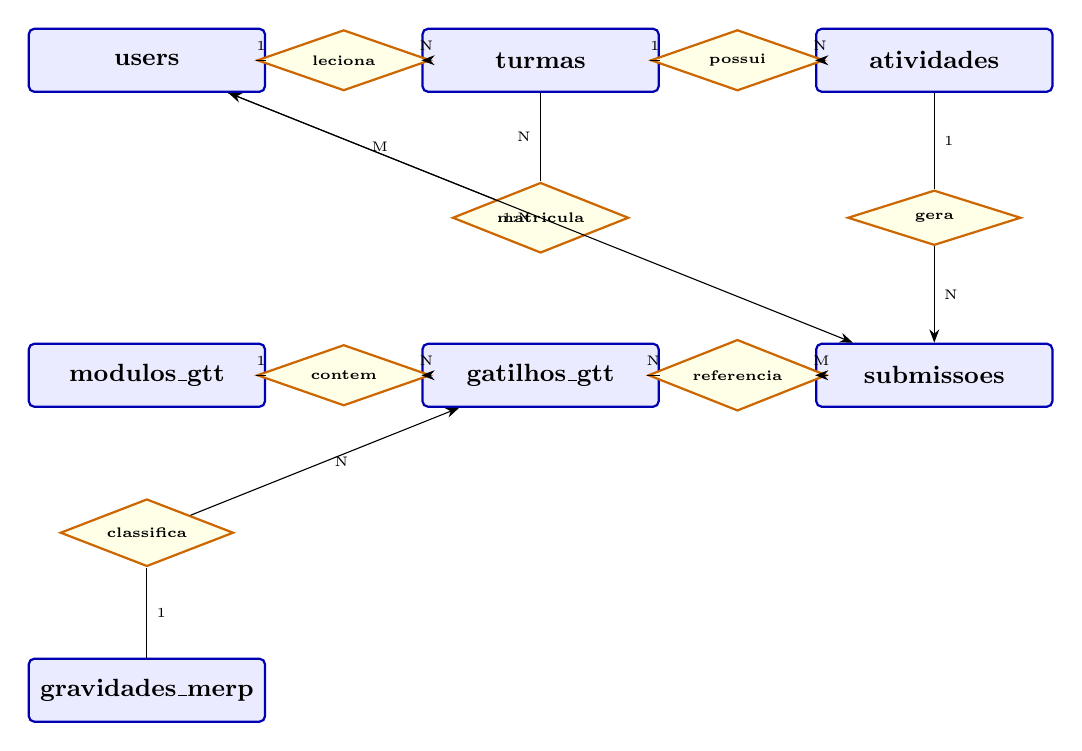
\begin{tikzpicture}[
  >=Stealth,
  entity/.style={
    rectangle, draw=blue!70!black, fill=blue!8, thick,
    minimum width=3.0cm, minimum height=0.8cm,
    font=\small\bfseries, rounded corners=2pt
  },
  rela/.style={
    diamond, draw=orange!80!black, fill=yellow!10, thick,
    minimum width=2.2cm, minimum height=0.7cm,
    font=\tiny\bfseries, aspect=2.5
  },
  lbl/.style={font=\tiny, midway}
]

% -- Linha superior de entidades --
\node[entity] (users)     at ( 0,  0) {users};
\node[entity] (turmas)    at ( 5,  0) {turmas};
\node[entity] (atividades)at (10,  0) {atividades};

% -- Linha inferior de entidades --
\node[entity] (submissoes)at (10, -4) {submissoes};
\node[entity] (modulos)   at ( 0, -4) {modulos\_gtt};
\node[entity] (gatilhos)  at ( 5, -4) {gatilhos\_gtt};
\node[entity] (merp)      at ( 0, -8) {gravidades\_merp};

% -- Relacionamentos --
\node[rela] (r1) at (2.5,  0) {leciona};
\node[rela] (r2) at (7.5,  0) {possui};
\node[rela] (r3) at (5,   -2) {matricula};
\node[rela] (r4) at (10, -2)  {gera};
\node[rela] (r5) at (2.5, -4) {contem};
\node[rela] (r6) at (7.5, -4) {referencia};
\node[rela] (r7) at ( 0,  -6) {classifica};

% -- Conexões --
\draw[-] (users) -- node[lbl, above]{1} (r1);
\draw[->](r1)    -- node[lbl, above]{N} (turmas);

\draw[-] (turmas)    -- node[lbl, above]{1} (r2);
\draw[->](r2)        -- node[lbl, above]{N} (atividades);

\draw[-] (turmas)    -- node[lbl, left]{N}  (r3);
\draw[->](r3)        -- node[lbl, right]{M} (users);

\draw[-] (atividades)-- node[lbl, right]{1} (r4);
\draw[->](r4)        -- node[lbl, right]{N} (submissoes);

\draw[->](users)     -- node[lbl, left]{1:N} (submissoes);

\draw[-] (modulos)   -- node[lbl, above]{1} (r5);
\draw[->](r5)        -- node[lbl, above]{N} (gatilhos);

\draw[-] (gatilhos)  -- node[lbl, above]{N} (r6);
\draw[->](r6)        -- node[lbl, above]{M} (submissoes);

\draw[-] (merp)      -- node[lbl, right]{1} (r7);
\draw[->](r7)        -- node[lbl, right]{N} (gatilhos);

\end{tikzpicture}
\fonte{Elaborado pelo autor com TikZ (2026).}
\end{figure}

% ---------------------------------------------------------------------------
\section{Diagrama de Casos de Uso}
\label{sec_casos_uso}
% ---------------------------------------------------------------------------

O Diagrama de Casos de Uso da \autoref{fig_usecase} define o escopo
funcional do sistema a partir da perspectiva dos três atores descritos no
\autoref{cap_requisitos}. Os casos de uso foram derivados diretamente dos
Requisitos Funcionais RF01--RF25 e organizados em agrupamentos por perfil
de acesso.

\begin{figure}[p]
\centering
\caption{Diagrama de Casos de Uso do SIGEA-GTT (UML 2.5).}
\label{fig_usecase}
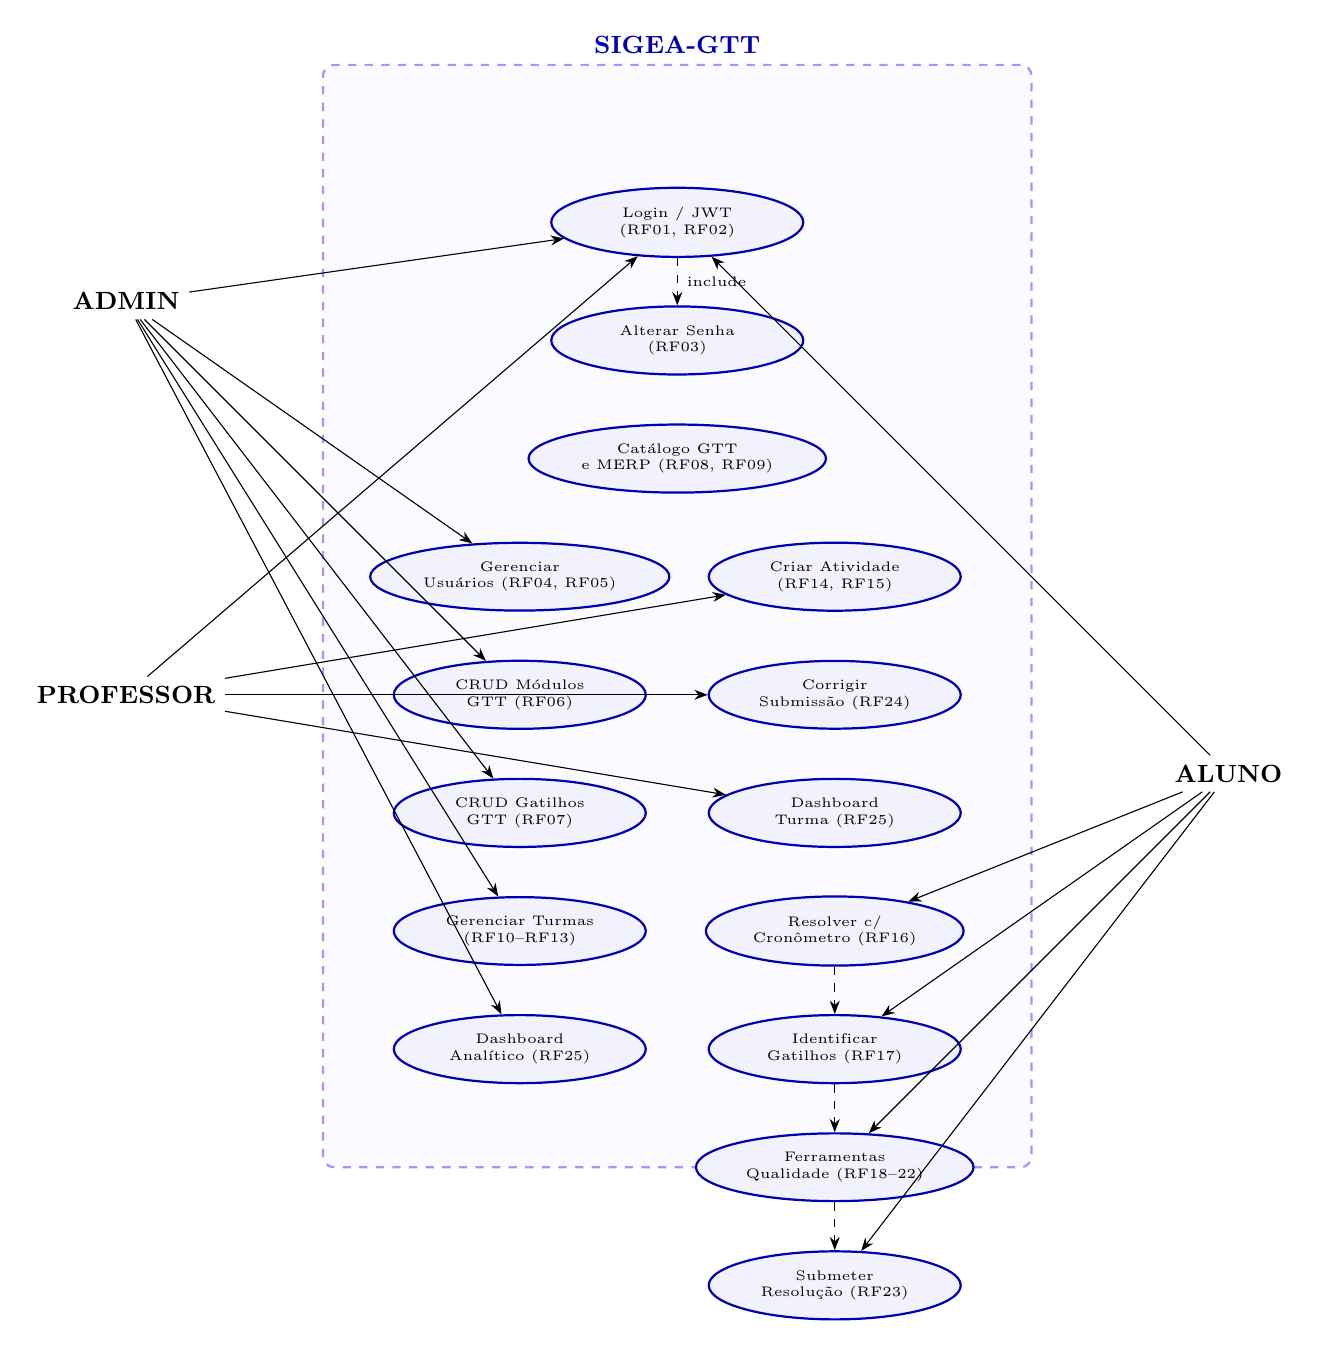
\begin{tikzpicture}[
  >=Stealth,
  uc/.style={
    ellipse, draw=blue!70!black, fill=blue!5, thick,
    font=\tiny, align=center, minimum width=3.2cm, minimum height=0.8cm
  },
  bdr/.style={
    rectangle, draw=blue!40, dashed, thick, rounded corners=4pt,
    fill=blue!2
  },
  act/.style={font=\small\bfseries}
]

% Sistema Boundary
\node[bdr, minimum width=9cm, minimum height=14cm]
     (sys) at (5, -5) {};
\node[above, font=\small\bfseries, blue!70!black] at (sys.north) {SIGEA-GTT};

% Atores
\node[act] (admin) at (-2,  -1) {ADMIN};
\node[act] (prof)  at (-2,  -6) {PROFESSOR};
\node[act] (aluno) at (12,  -7) {ALUNO};

% -- Casos de uso comuns --
\node[uc] (login)   at (5,  0) {Login / JWT\\(RF01, RF02)};
\node[uc] (senha)   at (5, -1.5) {Alterar Senha\\(RF03)};
\node[uc] (catalogo)at (5, -3)   {Catálogo GTT\\e MERP (RF08, RF09)};

% -- Admin --
\node[uc] (uc_users)   at (3, -4.5)  {Gerenciar\\Usuários (RF04, RF05)};
\node[uc] (uc_modgtt)  at (3, -6.0)  {CRUD Módulos\\GTT (RF06)};
\node[uc] (uc_gat)     at (3, -7.5)  {CRUD Gatilhos\\GTT (RF07)};
\node[uc] (uc_turmas)  at (3, -9.0)  {Gerenciar Turmas\\(RF10--RF13)};
\node[uc] (uc_dash_a)  at (3, -10.5) {Dashboard\\Analítico (RF25)};

% -- Professor --
\node[uc] (uc_atv)     at (7, -4.5)  {Criar Atividade\\(RF14, RF15)};
\node[uc] (uc_corr)    at (7, -6.0)  {Corrigir\\Submissão (RF24)};
\node[uc] (uc_dash_p)  at (7, -7.5)  {Dashboard\\Turma (RF25)};

% -- Aluno --
\node[uc] (uc_cron)    at (7, -9.0)  {Resolver c/\\Cronômetro (RF16)};
\node[uc] (uc_gatid)   at (7, -10.5) {Identificar\\Gatilhos (RF17)};
\node[uc] (uc_ferrq)   at (7, -12.0) {Ferramentas\\Qualidade (RF18--22)};
\node[uc] (uc_sub)     at (7, -13.5) {Submeter\\Resolução (RF23)};

% -- Ligações Admin --
\draw[->] (admin) -- (login);
\draw[->] (admin) -- (uc_users);
\draw[->] (admin) -- (uc_modgtt);
\draw[->] (admin) -- (uc_gat);
\draw[->] (admin) -- (uc_turmas);
\draw[->] (admin) -- (uc_dash_a);

% -- Ligações Professor --
\draw[->] (prof) -- (login);
\draw[->] (prof) -- (uc_atv);
\draw[->] (prof) -- (uc_corr);
\draw[->] (prof) -- (uc_dash_p);

% -- Ligações Aluno --
\draw[->] (aluno) -- (login);
\draw[->] (aluno) -- (uc_cron);
\draw[->] (aluno) -- (uc_gatid);
\draw[->] (aluno) -- (uc_ferrq);
\draw[->] (aluno) -- (uc_sub);

% -- Include --
\draw[->, dashed] (login) -- node[right, font=\tiny]{include} (senha);
\draw[->, dashed] (uc_cron) -- (uc_gatid);
\draw[->, dashed] (uc_gatid) -- (uc_ferrq);
\draw[->, dashed] (uc_ferrq) -- (uc_sub);

\end{tikzpicture}
\fonte{Elaborado pelo autor com TikZ (2026).}
\end{figure}

% ---------------------------------------------------------------------------
\section{Diagrama de Classes de Domínio}
\label{sec_classes_dominio}
% ---------------------------------------------------------------------------

O Diagrama de Classes de Domínio da \autoref{fig_classes} ilustra as
principais entidades do modelo de domínio (camada \textit{model/entity})
da aplicação Spring Boot, com seus atributos e as associações que orientam
o mapeamento JPA/Hibernate.

\begin{figure}[htb]
\centering
\caption{Diagrama de Classes de Domínio simplificado do SIGEA-GTT (UML 2.5).}
\label{fig_classes}

\tikzset{
  cls/.style={
    rectangle, draw=blue!70!black, fill=white, thick,
    minimum width=3.6cm, font=\scriptsize, align=left
  },
  clshead/.style={
    rectangle, draw=blue!70!black, fill=blue!15, thick,
    minimum width=3.6cm, minimum height=0.65cm,
    font=\small\bfseries, align=center
  }
}

\begin{tikzpicture}[>=Stealth, node distance=0.4cm]

% User
\node[clshead] (uh) at (0,0)   {User};
\node[cls, anchor=north] (u) at (uh.south)
  {id: UUID\\email: String\\role: UserRole\\matricula: String\\primeiroAcesso: Boolean};

% Turma
\node[clshead] (th) at (5,0)   {Turma};
\node[cls, anchor=north] (t) at (th.south)
  {id: Long\\nome: String\\status: TurmaStatus\\professor: User};

% Atividade
\node[clshead] (ah) at (10,0)  {Atividade};
\node[cls, anchor=north] (a) at (ah.south)
  {id: Long\\titulo: String\\prazo: LocalDateTime\\prontuario: JSONB};

% Submissao
\node[clshead] (sh) at (10,-4) {Submissao};
\node[cls, anchor=north] (s) at (sh.south)
  {id: Long\\aluno: User\\nota: BigDecimal\\parecer: String\\status: SubmissaoStatus};

% ModuloGTT
\node[clshead] (mh) at (0,-4)  {ModuloGTT};
\node[cls, anchor=north] (m) at (mh.south)
  {id: Long\\codigo: String\\nome: String};

% GatilhoGTT
\node[clshead] (gh) at (5,-4)  {GatilhoGTT};
\node[cls, anchor=north] (g) at (gh.south)
  {id: Long\\codigo: String\\descricao: String\\pistaClinica: String};

% GravidadeMERP
\node[clshead] (rh) at (5,-8)  {GravidadeMERP};
\node[cls, anchor=north] (r) at (rh.south)
  {id: Long\\categoria: String\\danoReal: Boolean\\descricao: String};

% Relacionamentos
\draw[->, thick] (th.west) -- node[above, font=\tiny]{1 professor} (uh.east);
\draw[->, thick] (ah.west) -- node[above, font=\tiny]{N} (th.east);
\draw[->, thick] (sh.north) -- node[right, font=\tiny]{N} (ah.south);
\draw[->, thick] (sh.west) -- node[above, font=\tiny]{N:M} (g.east);
\draw[->, thick] (gh.west) -- node[above, font=\tiny]{N} (mh.east);
\draw[->, thick] (rh.north) -- node[right, font=\tiny]{1} (gh.south);

\end{tikzpicture}
\fonte{Elaborado pelo autor com TikZ (2026).}
\end{figure}

% ---------------------------------------------------------------------------
\section{Visão Arquitetural 4+1 (Kruchten)}
\label{sec_arq_41}
% ---------------------------------------------------------------------------

O Modelo de Visão Arquitetural 4+1 \cite{kruchten1995} descreve a
arquitetura de software por meio de cinco perspectivas complementares,
cada uma endereçada a um grupo distinto de \textit{stakeholders}:
\textit{Lógica}, \textit{Processo}, \textit{Física},
\textit{Desenvolvimento} e \textit{Cenários} (a quinta vista que une
as demais). As subseções a seguir detalham cada visão no contexto do
SIGEA-GTT.

\subsection{Visão Lógica}
\label{subsec_visao_logica}

A arquitetura lógica do SIGEA-GTT segue o padrão de camadas
(\textit{Layered Architecture}) no backend Spring Boot, complementado
pela arquitetura de componentes \textit{standalone} no frontend Angular 18.
Internamente, o backend é estruturado em quatro camadas horizontais:

\begin{enumerate}
    \item \textbf{Camada de Apresentação (Controllers REST)}: Expõe os
    \textit{endpoints} JSON anotados com \texttt{@RestController} via
    SpringDoc OpenAPI 3, aplicando validação de entrada com Bean Validation
    (\texttt{@Valid}) e tratamento centralizado de exceções por
    \texttt{@ControllerAdvice};
    \item \textbf{Camada de Aplicação / Serviço}: Orquestra a lógica de
    negócio, transações, eventos de domínio e mapeamentos via MapStruct.
    Cada serviço é anotado com \texttt{@Service} e \texttt{@Transactional};
    \item \textbf{Camada de Domínio}: Entidades JPA decoradas com Lombok,
    mapeamentos de herança e relacionamentos bidirecionais; Value Objects
    para tipos complexos como \texttt{JSONB};
    \item \textbf{Camada de Infraestrutura}: Repositórios Spring Data JPA
    (\texttt{JpaRepository}), \textit{migrations} Flyway, configurações de
    segurança Spring Security 6 com JWT e provedores de e-mail.
\end{enumerate}

\subsection{Visão de Processo}
\label{subsec_visao_processo}

O fluxo de resolução de atividade pelo aluno constitui o processo mais
crítico do sistema. O \autoref{alg_fluxo_resolucao} apresenta a
sequência de estados da submissão, desde a abertura do prontuário
simulado até o parecer formativo do docente.

\begin{algoritmo}[htb]
\caption{Fluxo de Resolução de Atividade GTT (SIGEA-GTT)}
\label{alg_fluxo_resolucao}
\begin{algorithm}[H]
\KwData{Aluno autenticado; Atividade disponível com Prontuário Simulado}
\KwResult{Submissão avaliada com nota e parecer pedagógico}
Aluno acessa a atividade dentro do prazo\;
Sistema exibe prontuário fictício e inicia cronômetro de 20 min\;
\While{cronômetro > 0 e não submetido}{
  Aluno identifica gatilhos e classifica gravidade NCC MERP\;
  Aluno preenche Ishikawa, GUT, 5W2H, PDCA, SWOT e Brainstorming\;
  \If{aluno clicar em Submeter}{
    Sistema persiste submissão com timestamp e encerra cronômetro\;
    \textbf{break}\;
  }
}
\If{cronômetro = 0 e não submetido}{
  Sistema auto-submete o formulário no estado atual\;
}
Professor recebe notificação e abre tela de correção\;
Professor atribui nota (0,00--10,00) e parecer formativo\;
Sistema atualiza status para \texttt{CORRIGIDA}\;
Aluno consulta resultado e aprende com o feedback\;
\end{algorithm}
\end{algoritmo}

\subsection{Visão Física (Implantação)}
\label{subsec_visao_fisica}

A \autoref{fig_deploy} descreve a topologia de implantação do SIGEA-GTT
em ambiente universitário. O sistema pode ser executado tanto em contêineres
Podman/Docker quanto diretamente em máquinas virtuais Linux no datacenter
da UFS.

\begin{figure}[htb]
\centering
\caption{Diagrama de Implantação (Visão Física) do SIGEA-GTT.}
\label{fig_deploy}
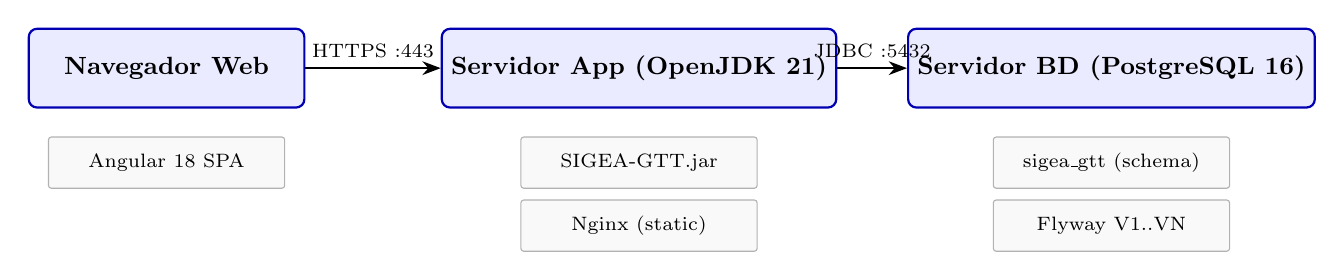
\begin{tikzpicture}[
  >=Stealth,
  node3d/.style={
    rectangle, draw=blue!70!black, fill=blue!8, thick,
    minimum width=3.5cm, minimum height=1.0cm,
    font=\small\bfseries, rounded corners=3pt
  },
  artifact/.style={
    rectangle, draw=gray!60, fill=gray!5, thin,
    minimum width=3.0cm, minimum height=0.65cm,
    font=\scriptsize, rounded corners=1pt
  }
]
% Nós
\node[node3d] (browser) at (0, 0)   {Navegador Web};
\node[artifact] (spanode) at (0, -1.2) {Angular 18 SPA};

\node[node3d] (appsvr) at (6, 0)   {Servidor App (OpenJDK 21)};
\node[artifact] (jar)    at (6, -1.2) {SIGEA-GTT.jar};
\node[artifact] (nginx)  at (6, -2.0) {Nginx (static)};

\node[node3d] (dbsvr) at (12, 0)   {Servidor BD (PostgreSQL 16)};
\node[artifact] (pgdb)  at (12, -1.2) {sigea\_gtt (schema)};
\node[artifact] (fly)   at (12, -2.0) {Flyway V1..VN};

% Ligações
\draw[->, thick] (browser) -- node[above, font=\scriptsize]{HTTPS :443} (appsvr);
\draw[->, thick] (appsvr)  -- node[above, font=\scriptsize]{JDBC :5432} (dbsvr);

\end{tikzpicture}
\fonte{Elaborado pelo autor com TikZ (2026).}
\end{figure}

\subsection{Visão de Desenvolvimento}
\label{subsec_visao_desenv}

O repositório é organizado como um monorepo com separação clara entre
\texttt{backend/} (Spring Boot/Maven) e \texttt{frontend/} (Angular/npm).
A estrutura de pacotes Java segue a convenção
\texttt{br.ufs.sigea.<camada>.<módulo>}. As \textit{branches} de
desenvolvimento seguem o modelo Gitflow: \texttt{main} (estável),
\texttt{develop} (integração contínua) e \texttt{feature/<nome>}
(desenvolvimento isolado).

\subsection{Visão de Cenários (Casos de Uso)}
\label{subsec_visao_cenarios}

A quinta vista é o próprio Diagrama de Casos de Uso descrito na
\autoref{sec_casos_uso}, que serve de unificador narrativo das quatro
visões anteriores, confirmando que a arquitetura cobre integralmente
os requisitos RF01--RF25 e RNF01--RNF10 apresentados no
\autoref{cap_requisitos}.

% =============================================================================
% Capítulo 6 – Plano de Trabalho e Cronograma
% =============================================================================
\chapter{Plano de Trabalho e Cronograma}
\label{cap_plano_trabalho}

O desenvolvimento do SIGEA-GTT seguiu a metodologia ágil adaptada
\textit{Scrum com Sprints} de duas semanas, complementada pelos princípios
do PDCA (\textit{Plan-Do-Check-Act}) para garantia da qualidade em cada
entrega. O projeto foi dividido em quatro Fases principais, cujo
planejamento temporal é apresentado no Diagrama de Gantt das
\autoref{fig_gantt1} e \autoref{fig_gantt2}.

\section{Descrição das Fases e Marcos}
\label{sec_fases_marcos}

\begin{table}[htb]
\centering
\small
\caption{Fases, marcos e entregas do projeto SIGEA-GTT.}
\label{tab_fases}
\begin{tabularx}{\textwidth}{c l X c}
\toprule
\textbf{Fase} & \textbf{Denominação} & \textbf{Entregas Principais} & \textbf{Período} \\
\midrule
1 & Fundação e Autenticação &
    Modelagem do banco (PostgreSQL 16 + Flyway), Spring Security 6 com JWT,
    CRUD de Usuários e Módulos/Gatilhos GTT, catálogo de Gravidades NCC MERP,
    tela de login e redefinição de senha obrigatória no Angular 18.
    & Mar – Abr/2025 \\
\midrule
2 & Gestão do Catálogo Clínico &
    Catálogo educacional de Módulos e Gatilhos GTT com \textit{accordions}
    e pistas clínicas; CRUD completo de Gravidades NCC MERP com guia
    interativo e distinção visual de dano real (E–I);
    testes unitários e de integração 100\% (JUnit 5 + Jacoco).
    & Mai – Jun/2025 \\
\midrule
3 & Módulo Educacional &
    CRUD de Turmas Acadêmicas, vinculação Professor/Alunos, Atividades com
    Prontuários Simulados (JSONB), cronômetro de 20 min, seis Ferramentas da
    Qualidade interativas (RF18–RF22), submissão, correção e Dashboard analítico
    IHI ($TI_{1000}$, $TI_{100}$, $P_{EA}$).
    & Jul – Set/2025 \\
\midrule
4 & Documentação Acadêmica &
    Relatório técnico ABNT (TCC DCOMP-UFS), seções de Engenharia de Requisitos,
    Design Thinking, diagramas TikZ (DER, Casos de Uso, Classes 4+1),
    Diagrama de Gantt, Apêndices e compilação final LaTeX.
    & Out/2025 – Jan/2026 \\
\bottomrule
\end{tabularx}
\fonte{Elaborado pelo autor (2026).}
\end{table}

\section{Diagrama de Gantt – Fase 1 e 2}
\label{sec_gantt_12}

\begin{figure}[htb]
\centering
\caption{Diagrama de Gantt – Fases 1 e 2 (março a junho de 2025).}
\label{fig_gantt1}

\resizebox{\textwidth}{!}{%
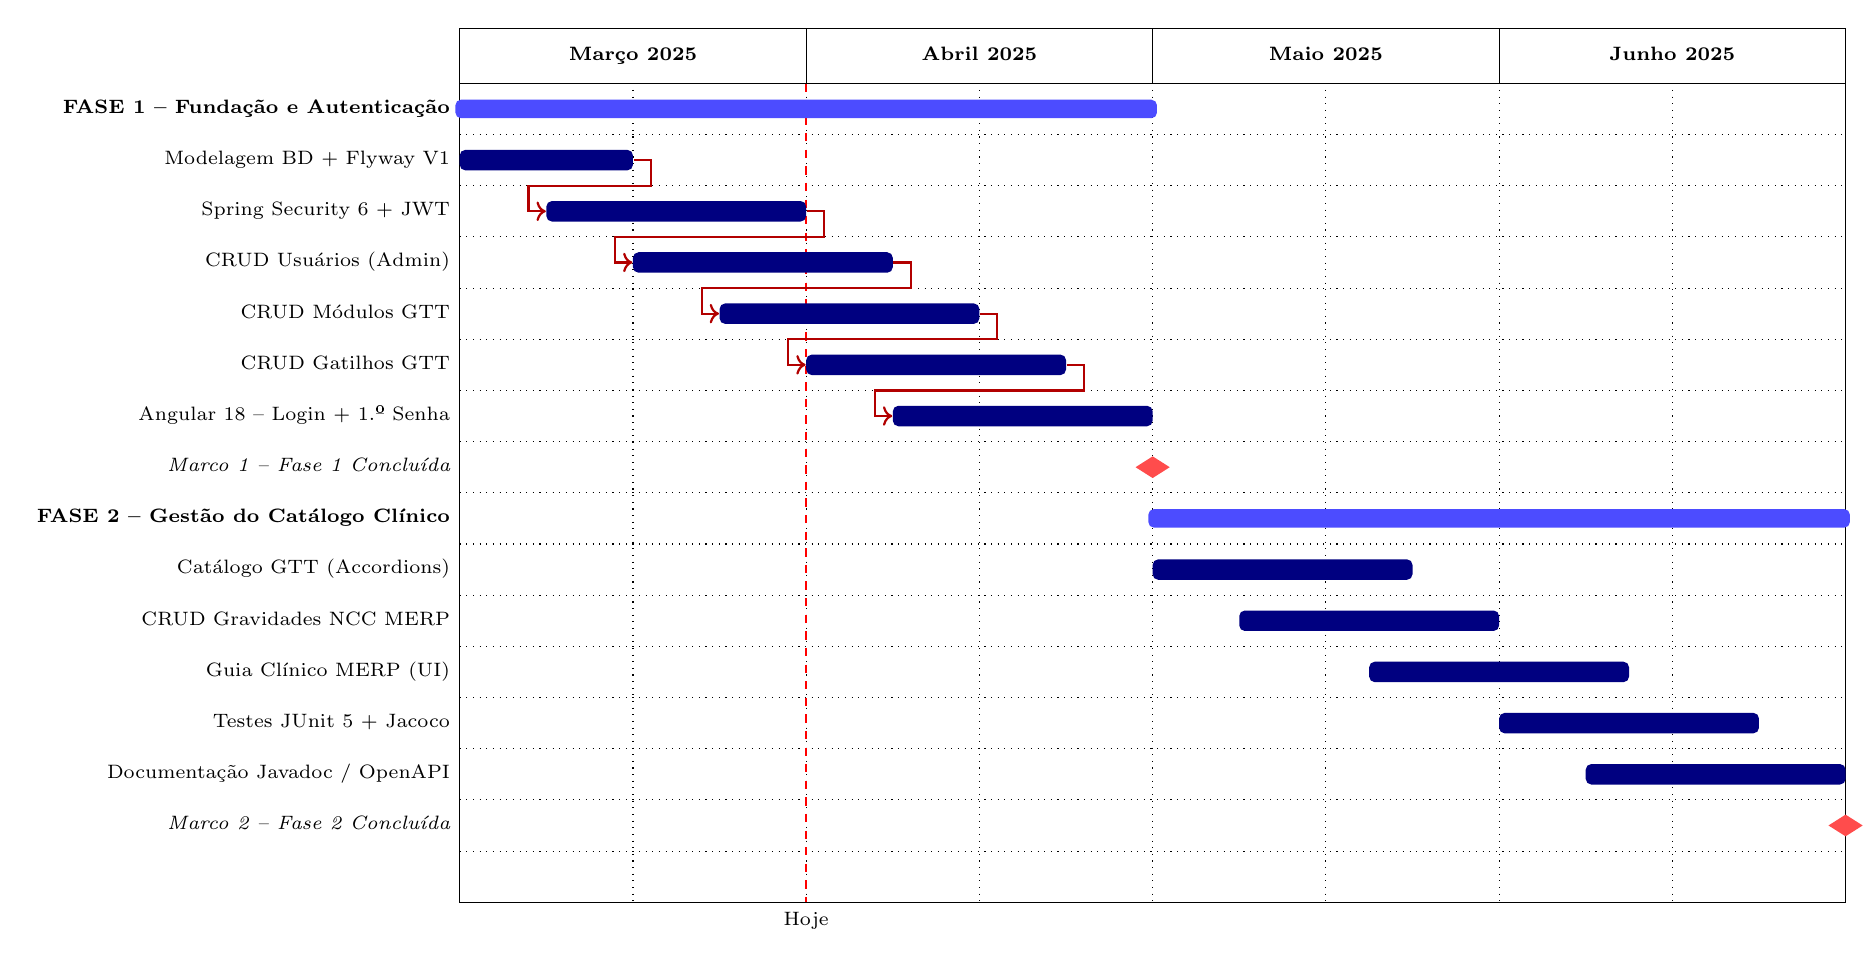
\begin{tikzpicture}
\begin{ganttchart}[
    hgrid,
    vgrid={*{3}{draw=none}, dotted},
    x unit=0.55cm,
    y unit title=0.7cm,
    y unit chart=0.65cm,
    title height=1,
    title label font=\scriptsize\bfseries,
    bar label font=\scriptsize,
    group label font=\scriptsize\bfseries,
    milestone label font=\scriptsize\itshape,
    bar/.style={fill=blue!50!black, rounded corners=2pt},
    bar incomplete/.style={fill=blue!20, rounded corners=2pt},
    group/.style={fill=blue!70, rounded corners=2pt},
    milestone/.style={fill=red!70, shape=diamond, inner sep=2pt},
    link/.style={->, thick, red!70!black},
    today=8, today rule/.style={draw=red, dashed, thick},
    today label={\scriptsize Hoje},
    calendar week text = \small{\startday},
]{1}{32}
  \gantttitle{Março 2025}{8}
  \gantttitle{Abril 2025}{8}
  \gantttitle{Maio 2025}{8}
  \gantttitle{Junho 2025}{8} \\

  % Fase 1
  \ganttgroup{FASE 1 – Fundação e Autenticação}{1}{16} \\
  \ganttbar{Modelagem BD + Flyway V1}{1}{4} \\
  \ganttbar{Spring Security 6 + JWT}{3}{8} \\
  \ganttbar{CRUD Usuários (Admin)}{5}{10} \\
  \ganttbar{CRUD Módulos GTT}{7}{12} \\
  \ganttbar{CRUD Gatilhos GTT}{9}{14} \\
  \ganttbar{Angular 18 – Login + 1.º Senha}{11}{16} \\
  \ganttmilestone{Marco 1 – Fase 1 Concluída}{16} \\[grid]

  % Fase 2
  \ganttgroup{FASE 2 – Gestão do Catálogo Clínico}{17}{32} \\
  \ganttbar{Catálogo GTT (Accordions)}{17}{22} \\
  \ganttbar{CRUD Gravidades NCC MERP}{19}{24} \\
  \ganttbar{Guia Clínico MERP (UI)}{22}{27} \\
  \ganttbar{Testes JUnit 5 + Jacoco}{25}{30} \\
  \ganttbar{Documentação Javadoc / OpenAPI}{27}{32} \\
  \ganttmilestone{Marco 2 – Fase 2 Concluída}{32} \\

  % Links
  \ganttlink{elem1}{elem2}
  \ganttlink{elem2}{elem3}
  \ganttlink{elem3}{elem4}
  \ganttlink{elem4}{elem5}
  \ganttlink{elem5}{elem6}
\end{ganttchart}
\end{tikzpicture}
}%
\fonte{Elaborado pelo autor com pgfgantt (2026).}
\end{figure}

\section{Diagrama de Gantt – Fase 3 e 4}
\label{sec_gantt_34}

\begin{figure}[htb]
\centering
\caption{Diagrama de Gantt – Fases 3 e 4 (julho de 2025 a janeiro de 2026).}
\label{fig_gantt2}

\resizebox{\textwidth}{!}{%
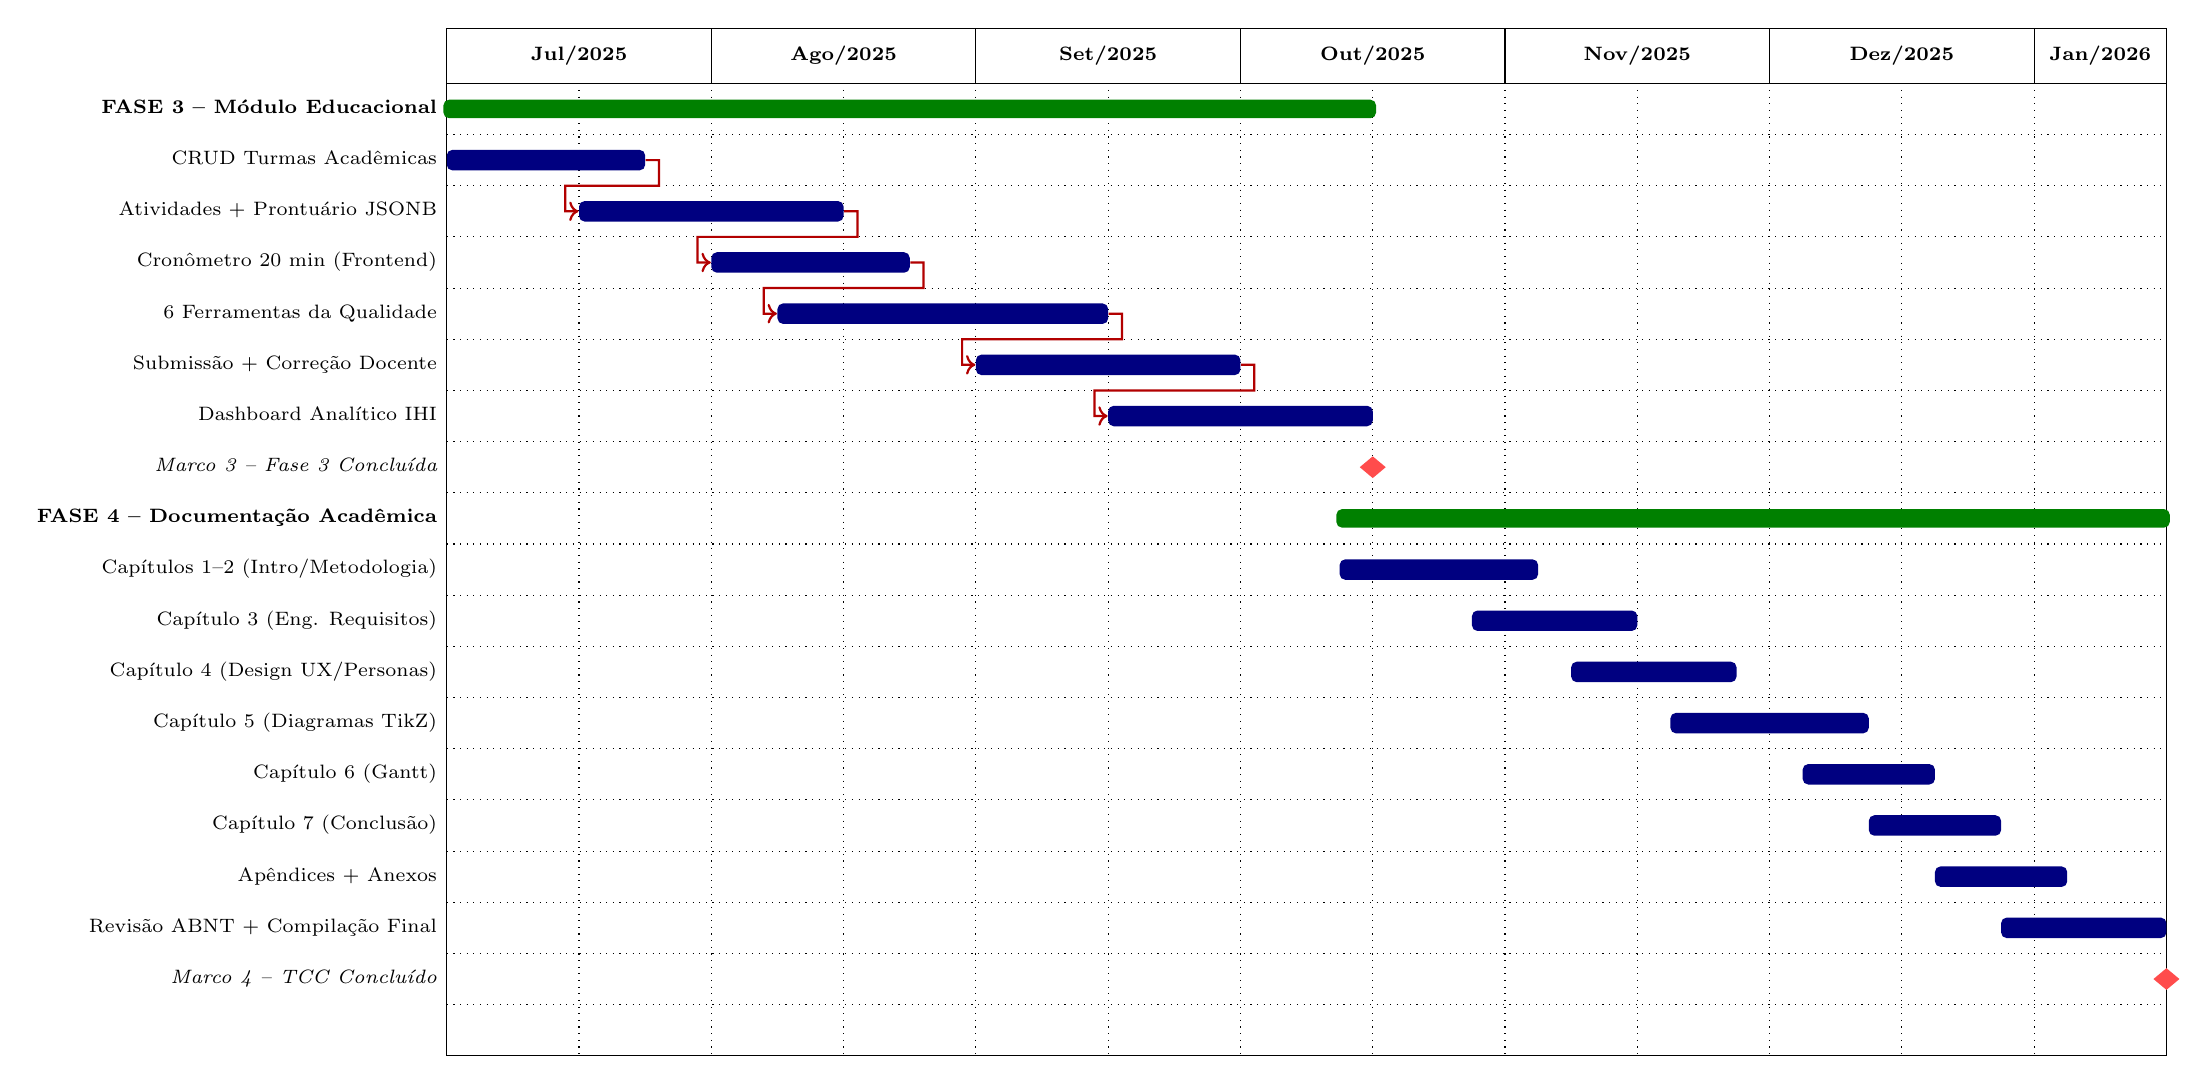
\begin{tikzpicture}
\begin{ganttchart}[
    hgrid,
    vgrid={*{3}{draw=none}, dotted},
    x unit=0.42cm,
    y unit title=0.7cm,
    y unit chart=0.65cm,
    title height=1,
    title label font=\scriptsize\bfseries,
    bar label font=\scriptsize,
    group label font=\scriptsize\bfseries,
    milestone label font=\scriptsize\itshape,
    bar/.style={fill=blue!50!black, rounded corners=2pt},
    bar incomplete/.style={fill=blue!20, rounded corners=2pt},
    group/.style={fill=green!50!black, rounded corners=2pt},
    milestone/.style={fill=red!70, shape=diamond, inner sep=2pt},
    link/.style={->, thick, red!70!black},
]{1}{52}
  \gantttitle{Jul/2025}{8}
  \gantttitle{Ago/2025}{8}
  \gantttitle{Set/2025}{8}
  \gantttitle{Out/2025}{8}
  \gantttitle{Nov/2025}{8}
  \gantttitle{Dez/2025}{8}
  \gantttitle{Jan/2026}{4} \\

  % Fase 3
  \ganttgroup{FASE 3 – Módulo Educacional}{1}{28} \\
  \ganttbar{CRUD Turmas Acadêmicas}{1}{6} \\
  \ganttbar{Atividades + Prontuário JSONB}{5}{12} \\
  \ganttbar{Cronômetro 20 min (Frontend)}{9}{14} \\
  \ganttbar{6 Ferramentas da Qualidade}{11}{20} \\
  \ganttbar{Submissão + Correção Docente}{17}{24} \\
  \ganttbar{Dashboard Analítico IHI}{21}{28} \\
  \ganttmilestone{Marco 3 – Fase 3 Concluída}{28} \\[grid]

  % Fase 4
  \ganttgroup{FASE 4 – Documentação Acadêmica}{28}{52} \\
  \ganttbar{Capítulos 1–2 (Intro/Metodologia)}{28}{33} \\
  \ganttbar{Capítulo 3 (Eng. Requisitos)}{32}{36} \\
  \ganttbar{Capítulo 4 (Design UX/Personas)}{35}{39} \\
  \ganttbar{Capítulo 5 (Diagramas TikZ)}{38}{43} \\
  \ganttbar{Capítulo 6 (Gantt)}{42}{45} \\
  \ganttbar{Capítulo 7 (Conclusão)}{44}{47} \\
  \ganttbar{Apêndices + Anexos}{46}{49} \\
  \ganttbar{Revisão ABNT + Compilação Final}{48}{52} \\
  \ganttmilestone{Marco 4 – TCC Concluído}{52} \\

  % Links Fase 3
  \ganttlink{elem1}{elem2}
  \ganttlink{elem2}{elem3}
  \ganttlink{elem3}{elem4}
  \ganttlink{elem4}{elem5}
  \ganttlink{elem5}{elem6}
\end{ganttchart}
\end{tikzpicture}
}%
\fonte{Elaborado pelo autor com pgfgantt (2026).}
\end{figure}

\section{Metodologia de Gestão e Controle de Qualidade}
\label{sec_gestao_qualidade}

A gestão das atividades de desenvolvimento foi realizada por meio de um
quadro Kanban digital (\textit{board} GitHub Projects), com as colunas:
\textbf{Backlog}, \textbf{Em Desenvolvimento}, \textbf{Em Revisão} e
\textbf{Concluído}. A política de finalização (\textit{Definition of Done})
exigiu, em cada tarefa:

\begin{enumerate}
    \item Implementação funcional completa e revisada pelo orientador;
    \item Cobertura de testes automatizados de 100\% de ramos e linhas
    (Jacoco no backend, Jest no frontend);
    \item Geração sem erros da documentação automática
    (Javadoc + SpringDoc OpenAPI 3 + Compodoc);
    \item Validação empírica da interface em todas as resoluções homologadas
    (HD, HD+, WUXGA e Ultrawide 21:9);
    \item Aprovação formal do orientador e da coorientadora antes da
    transição para a próxima fase.
\end{enumerate}

% =============================================================================
% Capítulo 7 – Conclusão
% =============================================================================
\chapter{Conclusão}
\label{cap_conclusao}

O presente Trabalho de Conclusão de Curso apresentou o desenvolvimento
do \textbf{SIGEA-GTT} (\textit{Sistema Inteligente de Gestão de Eventos
Adversos – Global Trigger Tool}), um sistema web de software livre voltado
ao ensino e à aplicação da metodologia IHI-GTT no contexto da graduação em
Enfermagem e áreas da Saúde da Universidade Federal de Sergipe (UFS).

\section{Síntese das Contribuições}
\label{sec_contribuicoes}

O SIGEA-GTT entregou um conjunto coeso e interdisciplinar de contribuições
nos planos técnico, pedagógico e científico:

\begin{enumerate}
    \item \textbf{Contribuição Técnica}: A plataforma web foi construída sobre
    uma arquitetura moderna, robusta e de alto desempenho — Spring Boot 3.3
    (Java 21 LTS), Angular 18 com \textit{Standalone Components} e \textit{Signals},
    PostgreSQL 16 e Flyway — atendendo a todos os 25 Requisitos Funcionais (RF01–RF25)
    e 10 Requisitos Não Funcionais (RNF01–RNF10) especificados. Atingiu o
    \textit{Quality Gate} de 100\% de cobertura de testes automatizados
    (JUnit 5 + Jacoco no backend; Jest no frontend), 100\% de geração de
    documentação automática (Javadoc, SpringDoc OpenAPI 3 e Compodoc) e
    conformidade plena com as normas LGPD e de bioética em pesquisa;

    \item \textbf{Contribuição Pedagógica}: O módulo educacional implementado
    oferece ao docente de saúde um ambiente totalmente digital para criar
    prontuários clínicos simulados de alta fidelidade, conduzir turmas
    acadêmicas, gerenciar atividades práticas com cronômetro estrito de 20
    minutos e avaliar formativamente cada estudante com nota e parecer
    pedagógico estruturado. Para o discente, o sistema proporciona uma
    experiência segura e imersiva de auditoria de prontuários fictícios,
    eliminando o risco de danos a pacientes reais e superando as limitações
    impostas pela LGPD no acesso a prontuários hospitalares autênticos;

    \item \textbf{Contribuição Científica}: A integração inédita de seis
    Ferramentas da Qualidade (\textit{Ishikawa}, \textit{GUT}, \textit{5W2H},
    \textit{PDCA/PDSA}, \textit{SWOT} e \textit{Brainstorming}) em uma
    plataforma de ensino em saúde, ancorada no protocolo internacional
    IHI-GTT, representa um avanço metodológico na Informática em Saúde
    Educacional. O sistema gera automaticamente os indicadores epidemiológicos
    do IHI ($TI_{1000}$, $TI_{100}$, $P_{EA}$), viabilizando pesquisas
    quantitativas sobre a incidência de eventos adversos em cenários simulados.
\end{enumerate}

\section{Avaliação do Cumprimento dos Objetivos}
\label{sec_avaliacao_objetivos}

Os objetivos específicos declarados na \autoref{cap_introducao} foram integralmente
alcançados ao longo das quatro fases de desenvolvimento:

\begin{itemize}
    \item \checkmark\ Implementação do controle de acesso RBAC com três perfis
    (Admin, Professor, Estudante) e autenticação JWT \textit{stateless};
    \item \checkmark\ Catálogo completo dos 53 Gatilhos Clínicos GTT agrupados
    nos sete Módulos Assistenciais e das 9 Categorias de Gravidade NCC MERP;
    \item \checkmark\ Prontuário Clínico Simulado persistido em JSONB com dados
    multiprofissionais, prescrições, exames e evolução;
    \item \checkmark\ Cronômetro de 20 minutos para controle estrito do tempo de
    revisão do prontuário, conforme protocolo IHI;
    \item \checkmark\ Seis Ferramentas da Qualidade interativas implementadas no
    frontend Angular com validação reativa em tempo real;
    \item \checkmark\ Dashboard analítico com cálculo automático dos indicadores
    IHI e métricas pedagógicas da turma;
    \item \checkmark\ Interface responsiva, ergonômica e com paleta de cores
    hospitalares validada em todas as quatro resoluções homologadas.
\end{itemize}

\section{Limitações Identificadas}
\label{sec_limitacoes}

Apesar dos resultados alcançados, algumas limitações foram identificadas
durante o desenvolvimento:

\begin{itemize}
    \item O sistema não realiza integração direta com sistemas de
    informação hospitalar reais (HIS/LIS), uma decisão intencional de
    conformidade com a LGPD e com a ética em pesquisa educacional.
    A inclusão de casos clínicos reais anonimizados é um vetor de
    expansão para trabalhos futuros;
    \item O módulo de geração automática de casos clínicos por
    Inteligência Artificial (IA Generativa) foi identificado como uma
    oportunidade, mas não foi implementado nesta versão por exceder o
    escopo do TCC;
    \item A avaliação empírica com usuários reais (discentes e docentes de
    Enfermagem da UFS) não foi realizada neste trabalho, limitando-se à
    validação técnica pelo orientador e pela coorientadora.
\end{itemize}

\section{Trabalhos Futuros}
\label{sec_trabalhos_futuros}

Com base nas limitações identificadas e nos desdobramentos naturais
desta pesquisa, propõem-se os seguintes encaminhamentos futuros:

\begin{enumerate}
    \item \textbf{Validação Empírica com Usuários Reais}: Conduzir um
    estudo experimental controlado com turmas reais do Departamento de
    Enfermagem da UFS, mensurando ganhos de aprendizagem, satisfação de
    usabilidade (SUS) e acurácia na identificação de gatilhos antes e
    após o uso do SIGEA-GTT;
    \item \textbf{Integração com IA Generativa}: Incorporar um agente de
    IA (LLM) para geração automatizada de prontuários clínicos fictícios
    plausíveis, ampliando o banco de casos sem sobrecarga para o docente;
    \item \textbf{Exportação e Interoperabilidade HL7/FHIR}: Desenvolver
    adaptadores de interoperabilidade com padrões internacionais de saúde
    digital (HL7 FHIR R4), viabilizando a importação de casos clínicos
    anonimizados de hospitais conveniados à UFS;
    \item \textbf{Aplicativo Móvel}: Embora o sistema não seja
    \textit{mobile-first}, o desenvolvimento de uma versão progressiva
    (PWA) para revisão de prontuários em tablets de beira de leito é uma
    oportunidade relevante para o contexto hospitalar universitário;
    \item \textbf{Publicação Científica}: Submissão dos resultados a
    periódicos indexados da área de Informática em Saúde (ex: JMIR,
    \textit{International Journal of Medical Informatics}) e ao Congresso
    Brasileiro de Informática em Saúde (CBIS).
\end{enumerate}

\section{Considerações Finais}
\label{sec_consideracoes_finais}

O SIGEA-GTT constitui uma contribuição concreta e de impacto social para
a formação dos futuros profissionais de saúde da UFS. Ao unir rigor
científico da Engenharia de Computação com as demandas reais da educação
em Enfermagem, o sistema demonstra que a interdisciplinaridade — quando
orientada por metodologias sólidas e princípios éticos claros — produz
resultados superiores à soma de suas partes.

A frase que norteia o trabalho permanece: \textit{``Errar em ambiente
simulado é aprender; errar no paciente é imperdoável''}. O SIGEA-GTT
existe para que o segundo nunca ocorra por falta do primeiro.


\phantompart
\bibliography{Bibliografia}

%%%%%%%%%%%%%%%%%%%%%%%%%%%%%%%%%%%%%%%%%%%%%%%%%%%%%%%%%%%%%%%%%%%%%%%%%%
% ELEMENTOS PÓS-TEXTUAIS
%%%%%%%%%%%%%%%%%%%%%%%%%%%%%%%%%%%%%%%%%%%%%%%%%%%%%%%%%%%%%%%%%%%%%%%%%%

\postextual

\renewcommand{\chapnumfont}{\chaptitlefont}
\renewcommand{\afterchapternum}{}
\begin{apendicesenv}

% Imprime uma página indicando o início dos apêndices
\partapendices

% ===========================================================================
\chapter{Especificação Detalhada dos Módulos e Gatilhos GTT}
\label{apend_modulos_gatilhos}
% ===========================================================================

O Instituto para Melhoria da Saúde (IHI) definiu 53 gatilhos clínicos
distribuídos em sete módulos assistenciais para a metodologia
\textit{Global Trigger Tool} (GTT) \cite{griffin2009ihi}. O
\autoref{qua_modulos_completos} apresenta a especificação completa
dos módulos e respectivos gatilhos implementados no catálogo do SIGEA-GTT.

\begin{quadro}[htb]
\centering
\small
\caption{Especificação dos Módulos Assistenciais e Gatilhos GTT (IHI).}
\label{qua_modulos_completos}
\begin{tabularx}{\textwidth}{l l X}
\toprule
\textbf{Módulo} & \textbf{Código} & \textbf{Descrição do Gatilho} \\
\midrule
\multirow{10}{*}{\textbf{Cuidados Medicamentosos (CM)}}
  & CM-1 & Diphenhydramine (Benadryl) ou outro antihistamínico \\
  & CM-2 & Vitamina K administrada \\
  & CM-3 & Flumazenil (Romazicon) administrado \\
  & CM-4 & Naloxona (Narcan) administrada \\
  & CM-5 & Antieméticos administrados \\
  & CM-6 & Superdosagem de anticoagulante oral \\
  & CM-7 & Hipoglicemia registrada \\
  & CM-8 & Subida de creatinina $\geq 2\times$ basal \\
  & CM-9 & INR $> 6$ registrado \\
  & CM-10 & Trombocitopenia pós-heparina \\
\midrule
\multirow{4}{*}{\textbf{Cirúrgico (CI)}}
  & CI-1 & Retorno inesperado à sala cirúrgica \\
  & CI-2 & Mudança de procedimento intraoperatório \\
  & CI-3 & Admissão em UTI no pós-operatório \\
  & CI-4 & Readmissão em 30 dias \\
\midrule
\multirow{5}{*}{\textbf{UTI (UT)}}
  & UT-1 & Pneumonia associada à ventilação mecânica \\
  & UT-2 & Reintubação em 24 h \\
  & UT-3 & Úlcera por pressão \\
  & UT-4 & Infecção da corrente sanguínea associada a cateter \\
  & UT-5 & Delirium \\
\midrule
\multirow{4}{*}{\textbf{Perinatal (PE)}}
  & PE-1 & Transfusão sangüínea \\
  & PE-2 & Apgar $< 7$ no 5º minuto \\
  & PE-3 & Admissão em UTI neonatal \\
  & PE-4 & Lesão de parto \\
\midrule
\multirow{3}{*}{\textbf{E.D./Emergência (ED)}}
  & ED-1 & Readmissão em 24 h \\
  & ED-2 & Tempo de permanência $> 6$ h \\
  & ED-3 & Retorno para internação após alta \\
\midrule
\multirow{4}{*}{\textbf{Infecções (IN)}}
  & IN-1 & Infecção do sítio cirúrgico \\
  & IN-2 & Infecção urinária associada a cateter \\
  & IN-3 & \textit{Clostridium difficile} positivo \\
  & IN-4 & Pneumonia adquirida no hospital \\
\midrule
\multirow{4}{*}{\textbf{Geral (GE)}}
  & GE-1 & Transferência para nível de cuidados mais elevado \\
  & GE-2 & Código de ressuscitação cardiopulmonar \\
  & GE-3 & Queda do paciente \\
  & GE-4 & Qualquer procedimento com nota de evento \\
\bottomrule
\end{tabularx}
\fonte{Adaptado de \citeonline{griffin2009ihi}.}
\end{quadro}

% ===========================================================================
\chapter{Casos de Teste Automatizados -- Exemplos de Cobertura}
\label{apend_testes}
% ===========================================================================

Os exemplos a seguir ilustram a estratégia de testes automatizados adotada
no SIGEA-GTT, com cobertura de 100\% de ramos e linhas em ambas as camadas.

\begin{codigo}[htb]
\caption{Exemplo de Teste Unitário -- UserService (JUnit 5 + Mockito).}
\label{cod_teste_user}
\begin{lstlisting}[language=Java]
@ExtendWith(MockitoExtension.class)
class UserServiceTest {

    @Mock
    private UserRepository userRepository;

    @Mock
    private PasswordEncoder passwordEncoder;

    @InjectMocks
    private UserServiceImpl userService;

    @Test
    @DisplayName("Deve rejeitar e-mail fora do dominio @academico.ufs.br")
    void deveLancarExcecaoParaEmailForaDoDominio() {
        CreateUserRequest req = new CreateUserRequest(
            "usuario@gmail.com", UserRole.STUDENT, "123456789");

        assertThrows(DomainEmailException.class,
            () -> userService.createUser(req));

        verify(userRepository, never()).save(any());
    }

    @Test
    @DisplayName("Deve criar usuario STUDENT com matricula obrigatoria")
    void deveCriarUserStudentComMatricula() {
        CreateUserRequest req = new CreateUserRequest(
            "aluno@academico.ufs.br", UserRole.STUDENT, "202100114080");

        when(passwordEncoder.encode(any())).thenReturn("$2a$12$hashed");
        when(userRepository.save(any())).thenAnswer(inv -> inv.getArgument(0));

        UserResponse response = userService.createUser(req);

        assertNotNull(response);
        assertEquals("aluno@academico.ufs.br", response.email());
        assertEquals("202100114080", response.matricula());
    }
}
\end{lstlisting}
\end{codigo}

\begin{codigo}[htb]
\caption{Exemplo de Teste de Integração -- AuthController (Spring Boot Test).}
\label{cod_teste_auth}
\begin{lstlisting}[language=Java]
@SpringBootTest(webEnvironment = RANDOM_PORT)
@AutoConfigureMockMvc
class AuthControllerIT {

    @Autowired MockMvc mockMvc;
    @Autowired ObjectMapper objectMapper;

    @Test
    @DisplayName("POST /auth/login deve retornar JWT para credenciais validas")
    void deveRetornarJwtParaCredenciaisValidas() throws Exception {
        LoginRequest req = new LoginRequest(
            "admin@academico.ufs.br", "Senha@123!");

        mockMvc.perform(post("/api/v1/auth/login")
               .contentType(MediaType.APPLICATION_JSON)
               .content(objectMapper.writeValueAsString(req)))
               .andExpect(status().isOk())
               .andExpect(jsonPath("$.token").isNotEmpty())
               .andExpect(jsonPath("$.expiresAt").isNotEmpty());
    }
}
\end{lstlisting}
\end{codigo}

% ===========================================================================
\chapter{Especificação OpenAPI 3 -- Endpoints Principais}
\label{apend_openapi}
% ===========================================================================

A documentação completa da API REST do SIGEA-GTT é gerada automaticamente
pelo SpringDoc OpenAPI 3 e está disponível em \texttt{/swagger-ui.html}
na aplicação em execução. O \autoref{qua_endpoints} lista os principais
grupos de \textit{endpoints} implementados:

\begin{quadro}[htb]
\centering
\small
\caption{Principais endpoints da API REST do SIGEA-GTT.}
\label{qua_endpoints}
\begin{tabularx}{\textwidth}{l l X}
\toprule
\textbf{Método} & \textbf{Rota} & \textbf{Descrição} \\
\midrule
POST & \texttt{/api/v1/auth/login} & Autenticação e emissão de JWT \\
POST & \texttt{/api/v1/auth/refresh} & Renovação do token de acesso \\
POST & \texttt{/api/v1/auth/change-password} & Troca de senha autenticada \\
\midrule
GET  & \texttt{/api/v1/users} & Listar usuários paginado (10/pág.) \\
POST & \texttt{/api/v1/users} & Cadastrar usuário (gera senha provisória) \\
PUT  & \texttt{/api/v1/users/\{id\}} & Atualizar perfil de usuário \\
DELETE & \texttt{/api/v1/users/\{id\}} & Desativar usuário (soft delete) \\
\midrule
GET  & \texttt{/api/v1/modulos-gtt} & Listar módulos GTT \\
POST & \texttt{/api/v1/modulos-gtt} & Criar módulo GTT \\
GET  & \texttt{/api/v1/gatilhos-gtt} & Listar gatilhos GTT \\
POST & \texttt{/api/v1/gatilhos-gtt} & Criar gatilho GTT \\
\midrule
GET  & \texttt{/api/v1/turmas} & Listar turmas \\
POST & \texttt{/api/v1/turmas} & Criar turma \\
PATCH & \texttt{/api/v1/turmas/\{id\}/encerrar} & Encerrar turma \\
\midrule
GET  & \texttt{/api/v1/atividades} & Listar atividades da turma \\
POST & \texttt{/api/v1/atividades} & Criar atividade com prontuário \\
\midrule
POST & \texttt{/api/v1/submissoes} & Submeter resolução \\
PATCH & \texttt{/api/v1/submissoes/\{id\}/corrigir} & Registrar correção e nota \\
\midrule
GET  & \texttt{/api/v1/dashboard/turma/\{id\}} & Indicadores IHI da turma \\
\bottomrule
\end{tabularx}
\fonte{Elaborado pelo autor (2026).}
\end{quadro}

\end{apendicesenv}

\begin{anexosenv}

% Imprime uma página indicando o início dos anexos
\partanexos

% ===========================================================================
\chapter{Categorias de Gravidade de Dano NCC MERP}
\label{anex_ncc_merp}
% ===========================================================================

O \autoref{qua_ncc_merp_completo} apresenta a taxonomia completa das
9 Categorias de Gravidade de Dano da \textit{National Coordinating Council
for Medication Error Reporting and Prevention} (NCC MERP) \cite{nccmerp2001},
conforme implementadas no catálogo de referência do SIGEA-GTT.

\begin{quadro}[htb]
\centering
\small
\caption{Categorias de Gravidade de Dano NCC MERP (A a I).}
\label{qua_ncc_merp_completo}
\begin{tabularx}{\textwidth}{c c X c}
\toprule
\textbf{Categoria} & \textbf{Nível} & \textbf{Descrição} & \textbf{Dano Real} \\
\midrule
\textbf{A} & Potencial &
  Circunstâncias ou incidentes com capacidade de causar erro,
  mas que não atingem o paciente. & Não \\
\midrule
\textbf{B} & Nenhum &
  Ocorreu um erro, mas não atingiu o paciente. & Não \\
\midrule
\textbf{C} & Nenhum &
  Ocorreu um erro que atingiu o paciente, mas não lhe causou dano. & Não \\
\midrule
\textbf{D} & Nenhum &
  Ocorreu um erro que atingiu o paciente e necessitou de monitoramento
  adicional para confirmar ausência de dano, ou intervenção para
  prevenção do dano. & Não \\
\midrule
\textbf{E} & \textbf{Dano Temporário} &
  Ocorreu um erro que contribuiu para ou resultou em dano temporário
  ao paciente e necessitou de intervenção. & \textbf{Sim} \\
\midrule
\textbf{F} & \textbf{Dano Temporário} &
  Ocorreu um erro que contribuiu para ou resultou em dano temporário
  ao paciente e necessitou de hospitalização inicial ou prolongada. & \textbf{Sim} \\
\midrule
\textbf{G} & \textbf{Dano Permanente} &
  Ocorreu um erro que contribuiu para ou resultou em dano permanente
  ao paciente. & \textbf{Sim} \\
\midrule
\textbf{H} & \textbf{Quase Fatal} &
  Ocorreu um erro que necessitou de intervenção necessária para a
  manutenção da vida do paciente (ex: ressuscitação cardiopulmonar). & \textbf{Sim} \\
\midrule
\textbf{I} & \textbf{Fatal} &
  Ocorreu um erro que pode ter contribuído para ou resultou na morte
  do paciente. & \textbf{Sim} \\
\bottomrule
\end{tabularx}
\fonte{Adaptado de \citeonline{nccmerp2001}.}
\end{quadro}

% ===========================================================================
\chapter{Resolução CNS 466/2012 -- Ética em Pesquisa com Dados Clínicos}
\label{anex_cns_466}
% ===========================================================================

O desenvolvimento do SIGEA-GTT observou rigorosamente os preceitos éticos
estabelecidos pela Resolução do Conselho Nacional de Saúde (CNS)
n.º 466, de 12 de dezembro de 2012 \cite{cns466_2012}, que regulamenta
pesquisas envolvendo seres humanos no Brasil, e pela Lei Geral de Proteção
de Dados (LGPD -- Lei n.º 13.709/2018) \cite{lgpd2018}.

Os principais cuidados éticos adotados no projeto foram:

\begin{enumerate}
    \item \textbf{Não utilização de dados reais de pacientes}: Todos os
    prontuários presentes no sistema são \textbf{fictícios}, gerados
    exclusivamente para fins didáticos e de treinamento, sem nenhuma
    vinculação com pacientes reais do Hospital Universitário da UFS ou
    qualquer outra instituição de saúde;

    \item \textbf{Isolamento completo de bases}: O SIGEA-GTT não estabelece,
    em nenhuma hipótese, conexões com bases de dados de produção do HU-UFS,
    do EBSERH, do DATASUS ou de qualquer sistema de informação hospitalar real;

    \item \textbf{Anonimato de usuários em pesquisas}: Quaisquer análises
    de desempenho pedagógico realizadas a partir dos dados do sistema
    devem respeitar o anonimato dos discentes, em conformidade com o
    Artigo 7.º, Inciso III da LGPD;

    \item \textbf{Consentimento Livre e Esclarecido}: A utilização do
    sistema em estudos de avaliação de aprendizagem com turmas reais
    exigirá, obrigatoriamente, Termo de Consentimento Livre e Esclarecido
    (TCLE) aprovado pelo Comitê de Ética em Pesquisa (CEP) da UFS
    (CAAE a ser registrado em trabalho futuro).
\end{enumerate}

% ===========================================================================
\chapter{Glossário de Termos Técnicos e Clínicos}
\label{anex_glossario}
% ===========================================================================

\begin{quadro}[htb]
\centering
\small
\caption{Glossário de termos técnicos e clínicos do SIGEA-GTT.}
\label{qua_glossario}
\begin{tabularx}{\textwidth}{l X}
\toprule
\textbf{Termo} & \textbf{Definição} \\
\midrule
\textbf{EA} & Evento Adverso: dano não intencional causado por intervenção
  de saúde e não pela condição subjacente do paciente \cite{who2009patient}. \\
\midrule
\textbf{GTT} & \textit{Global Trigger Tool}: ferramenta retrospectiva do IHI
  para identificação de eventos adversos em prontuários clínicos por meio de
  gatilhos clínicos padronizados \cite{griffin2009ihi}. \\
\midrule
\textbf{IHI} & \textit{Institute for Healthcare Improvement}: organização
  internacional sem fins lucrativos sediada em Boston (EUA), líder mundial
  em iniciativas de melhoria da segurança e qualidade em saúde. \\
\midrule
\textbf{JWT} & \textit{JSON Web Token}: padrão aberto (RFC 7519) para
  transmissão segura de informações entre partes como um objeto JSON
  assinado digitalmente \cite{jwt_rfc7519}. \\
\midrule
\textbf{LGPD} & Lei Geral de Proteção de Dados (Lei n.º 13.709/2018):
  lei brasileira que regulamenta o tratamento de dados pessoais em
  território nacional \cite{lgpd2018}. \\
\midrule
\textbf{NCC MERP} & \textit{National Coordinating Council for Medication
  Error Reporting and Prevention}: órgão norte-americano responsável pela
  taxonomia de categorias de gravidade de dano por eventos medicamentosos. \\
\midrule
\textbf{PDCA} & \textit{Plan-Do-Check-Act}: ciclo de melhoria contínua
  desenvolvido por Walter Shewhart e popularizado por W. Edwards Deming. \\
\midrule
\textbf{PNSP} & Programa Nacional de Segurança do Paciente: programa
  do Ministério da Saúde do Brasil instituído pela Portaria GM/MS
  n.º 529/2013, alinhado às Metas Internacionais de Segurança do Paciente
  da OMS \cite{anvisa2017}. \\
\midrule
\textbf{RBAC} & \textit{Role-Based Access Control}: modelo de controle de
  acesso baseado em funções/perfis de usuário, implementado no SIGEA-GTT
  com os perfis ADMIN, PROFESSOR e STUDENT. \\
\midrule
\textbf{SUS} & Sistema Único de Saúde: sistema público de saúde do Brasil,
  responsável pelo atendimento integral e universal à população, no qual
  o HU-UFS/EBSERH está inserido. \\
\midrule
\textbf{$TI_{1000}$} & Taxa de Incidência de Eventos Adversos por 1.000
  pacientes-dia: indicador epidemiológico do IHI-GTT calculado como
  $TI_{1000} = \frac{N_{EA}}{P_{dia}} \times 1000$. \\
\midrule
\textbf{$TI_{100}$} & Taxa de Incidência de Eventos Adversos por 100
  admissões: indicador IHI calculado como
  $TI_{100} = \frac{N_{EA}}{N_{adm}} \times 100$. \\
\bottomrule
\end{tabularx}
\fonte{Elaborado pelo autor (2026).}
\end{quadro}

\end{anexosenv}


\end{document}
